\section{Supplementary Cohort Analysis}
\label{app:cohort_figures}

This appendix reports the complete multiscale topological analysis for the additional sEEG recordings in the dataset, obtained after applying extracranial channel filtering (\texttt{POL}/\texttt{ECG} removal), electrophysiological onset alignment ($t = 0\text{ s}$), and sub-critical baseline threshold calibration.

\subsection{Recording \texttt{DB470451}}
\label{app:rec_db470451}

\begin{figure}[htbp]
    \centering
    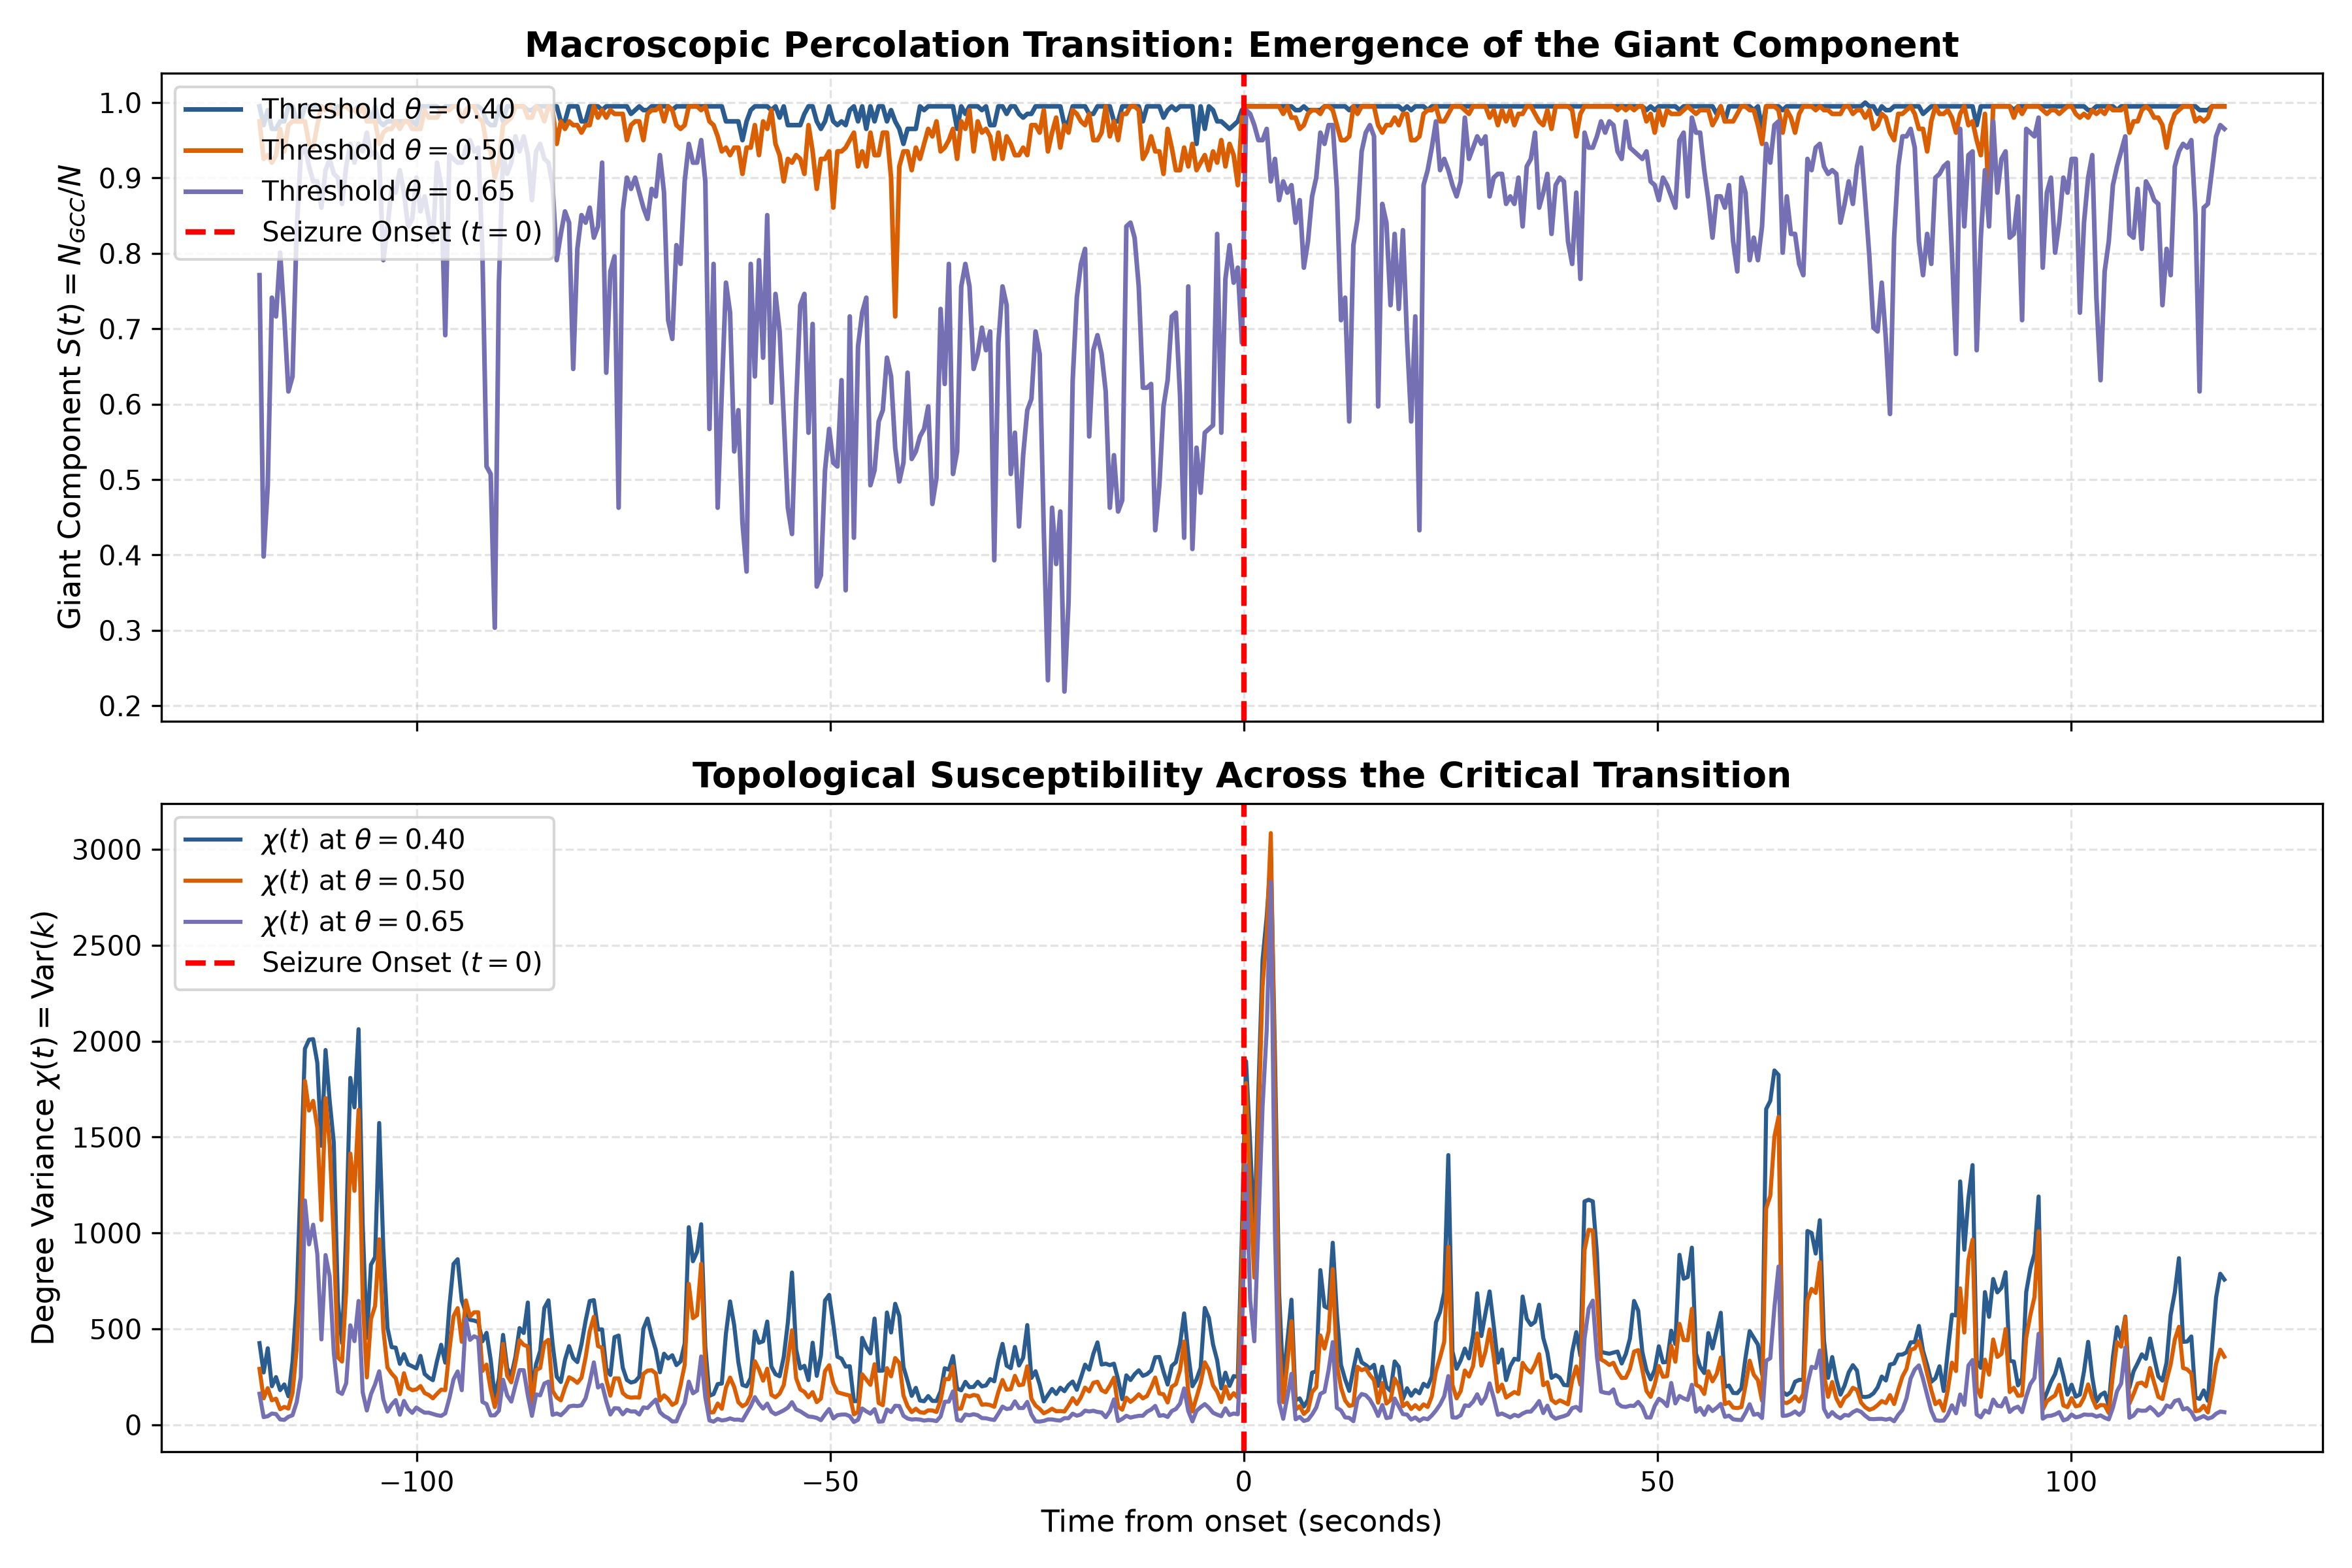
\includegraphics[width=0.8\textwidth]{img/DB470451/macro_percolation_transition.png}
    \caption{Macroscopic Percolation ($S(\tau)$ and $\chi(\tau)$) for recording \texttt{DB470451}.}
    \label{fig:db470451_macro}
\end{figure}

\begin{figure}[htbp]
    \centering
    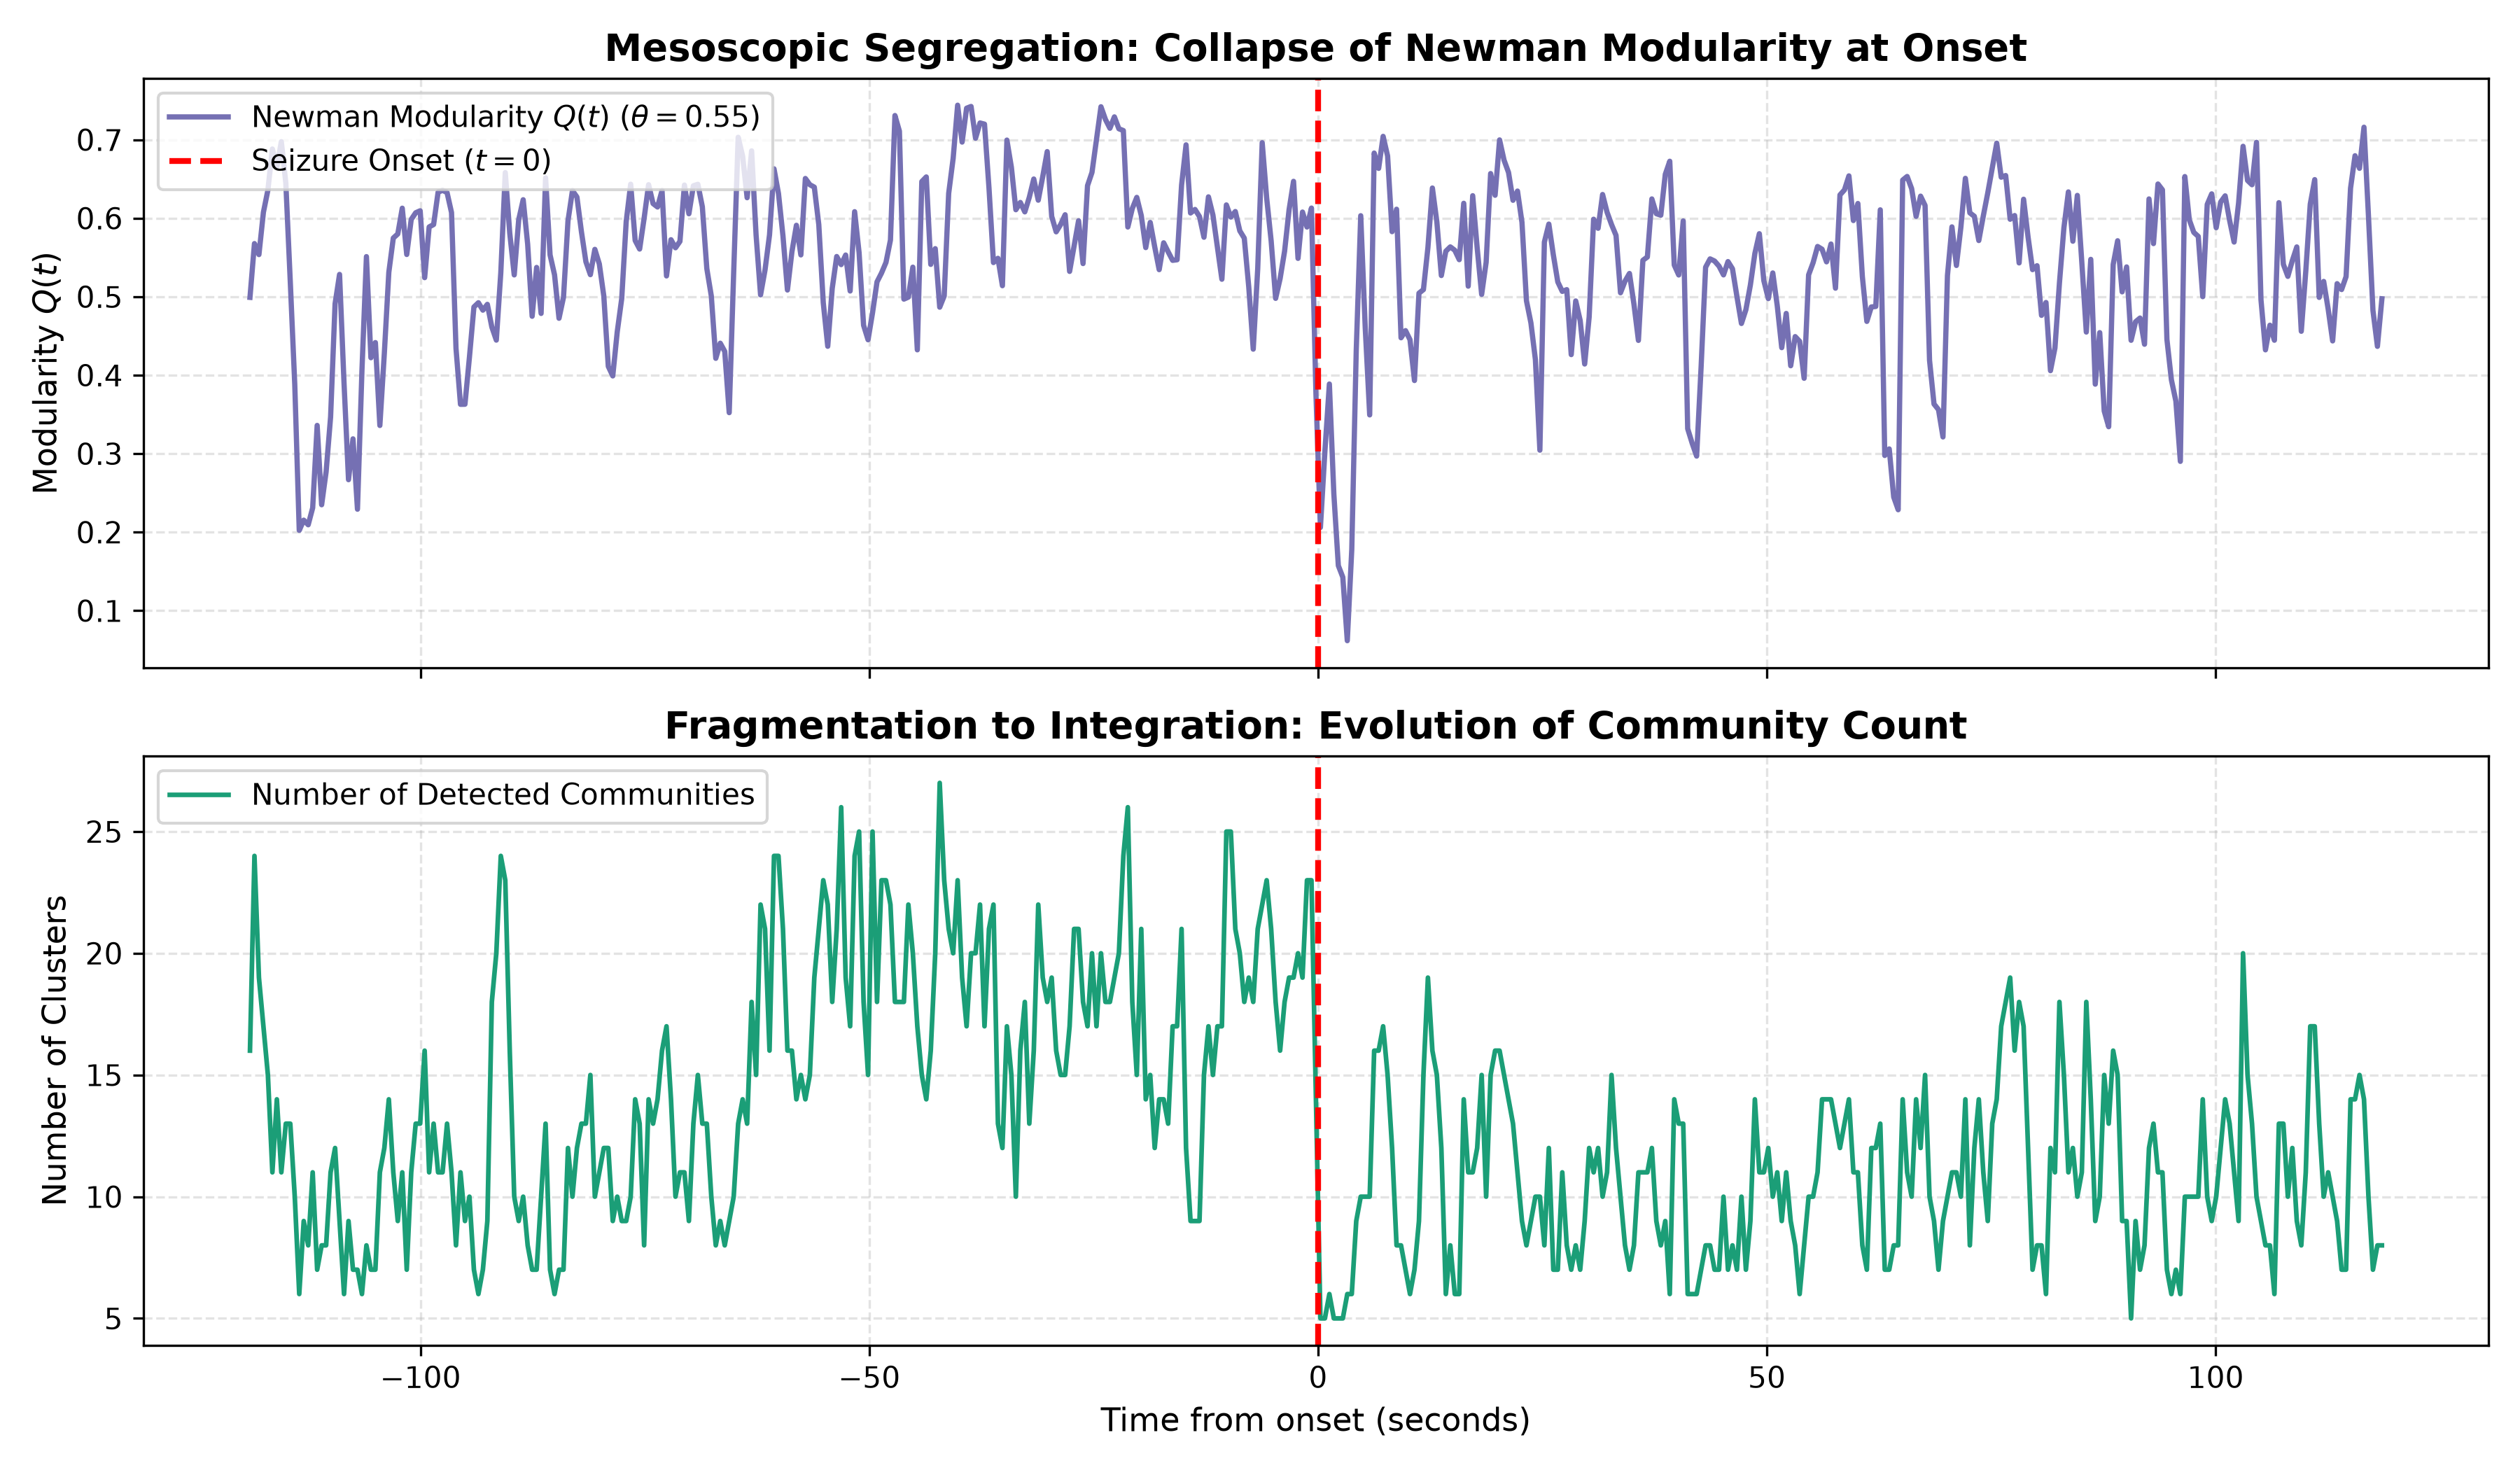
\includegraphics[width=0.8\textwidth]{img/DB470451/meso_modularity_collapse.png}
    \caption{Mesoscopic Modularity Collapse ($Q(\tau)$ and $N_c(\tau)$) for recording \texttt{DB470451}.}
    \label{fig:db470451_meso}
\end{figure}

\begin{figure}[htbp]
    \centering
    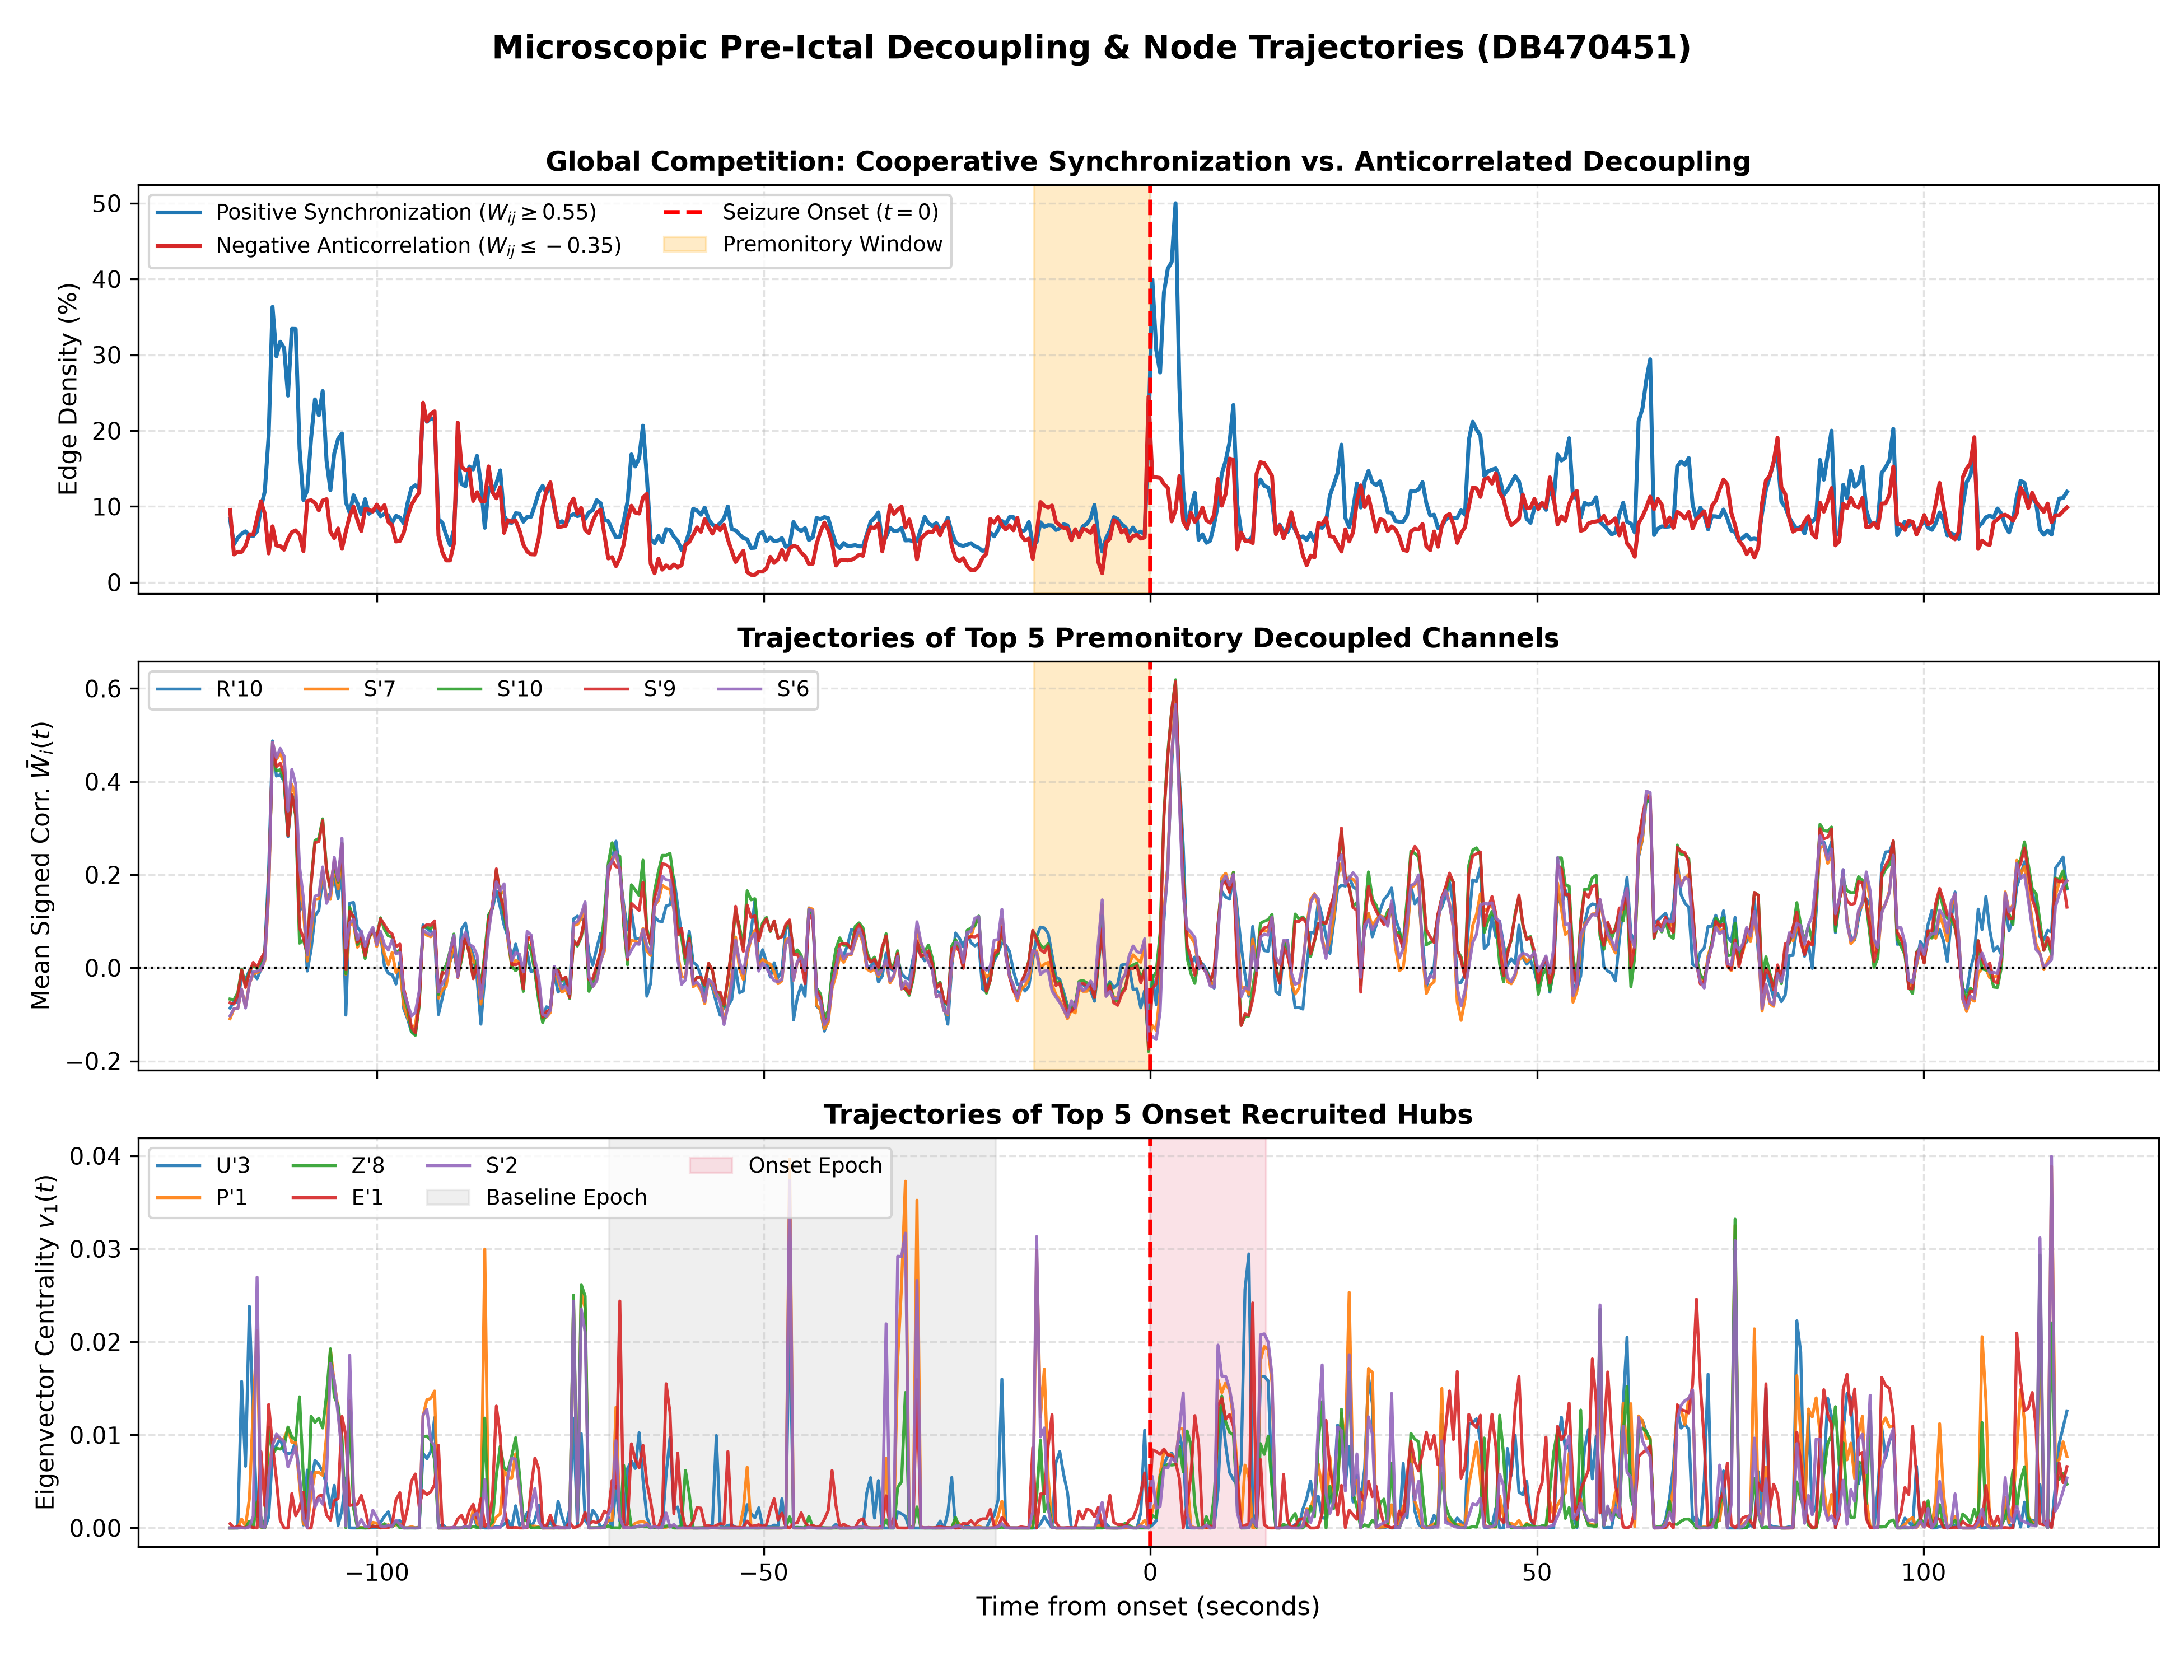
\includegraphics[width=0.8\textwidth]{img/DB470451/micro_premonitory_decoupling.png}
    \caption{Premonitory Decoupling and Hub Trajectories for recording \texttt{DB470451}.}
    \label{fig:db470451_micro_traj}
\end{figure}

\begin{figure}[htbp]
    \centering
    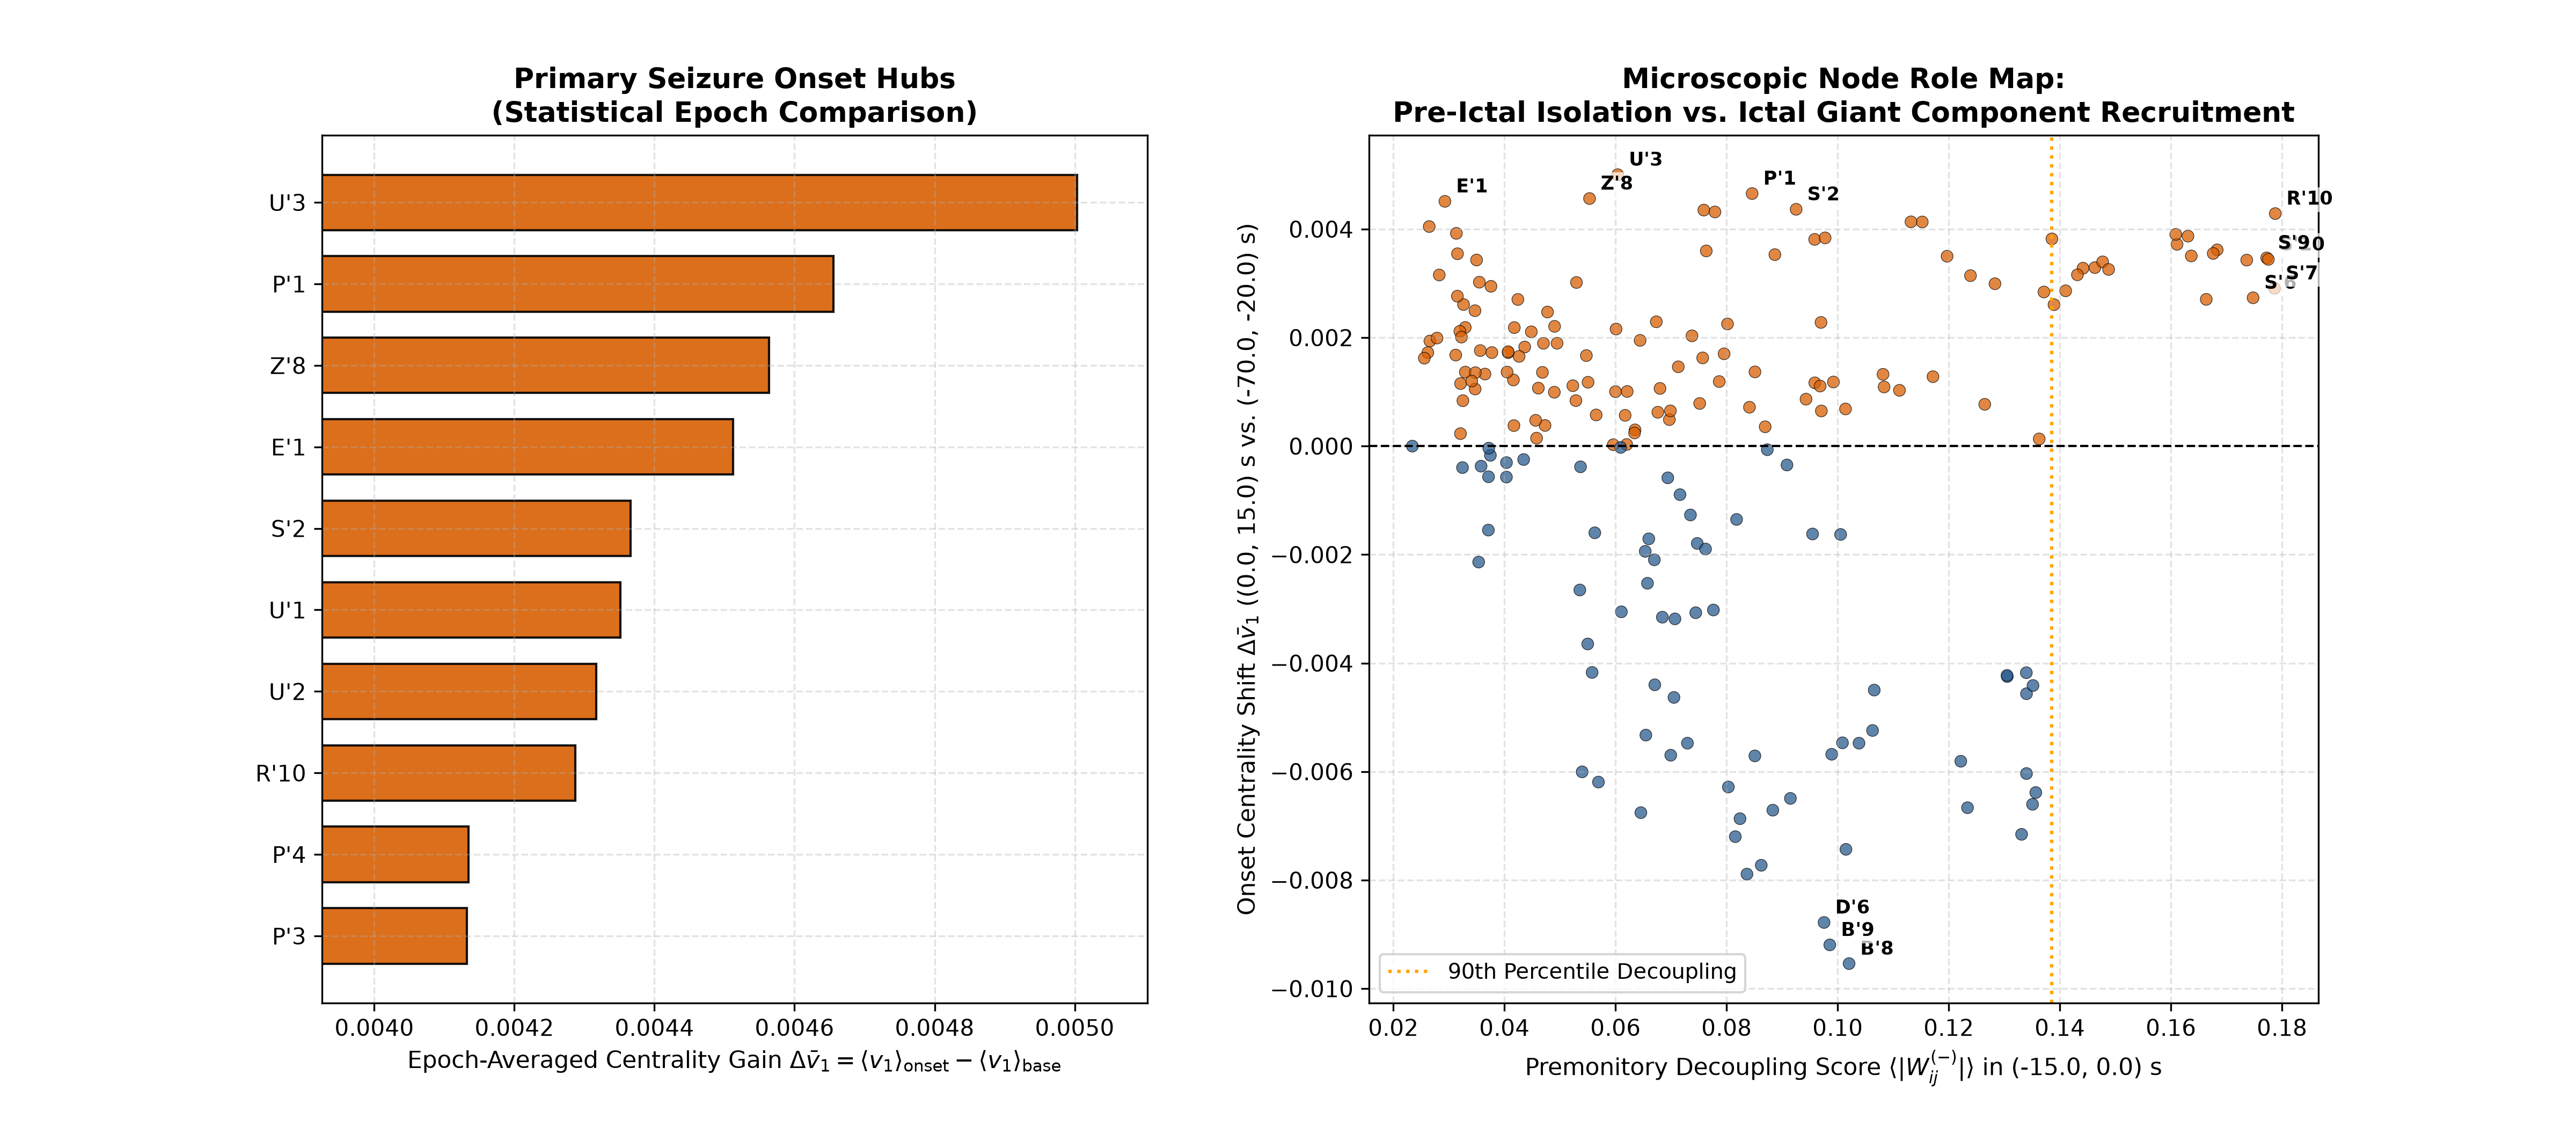
\includegraphics[width=0.9\textwidth]{img/DB470451/micro_hub_recruitment_and_roles.png}
    \caption{Onset Hub Ranking and 2D Functional Role Map for recording \texttt{DB470451}.}
    \label{fig:db470451_micro_roles}
\end{figure}

\clearpage

\subsection{Recording \texttt{DQ0040P6}}
\label{app:rec_dq0040p6}

\begin{figure}[htbp]
    \centering
    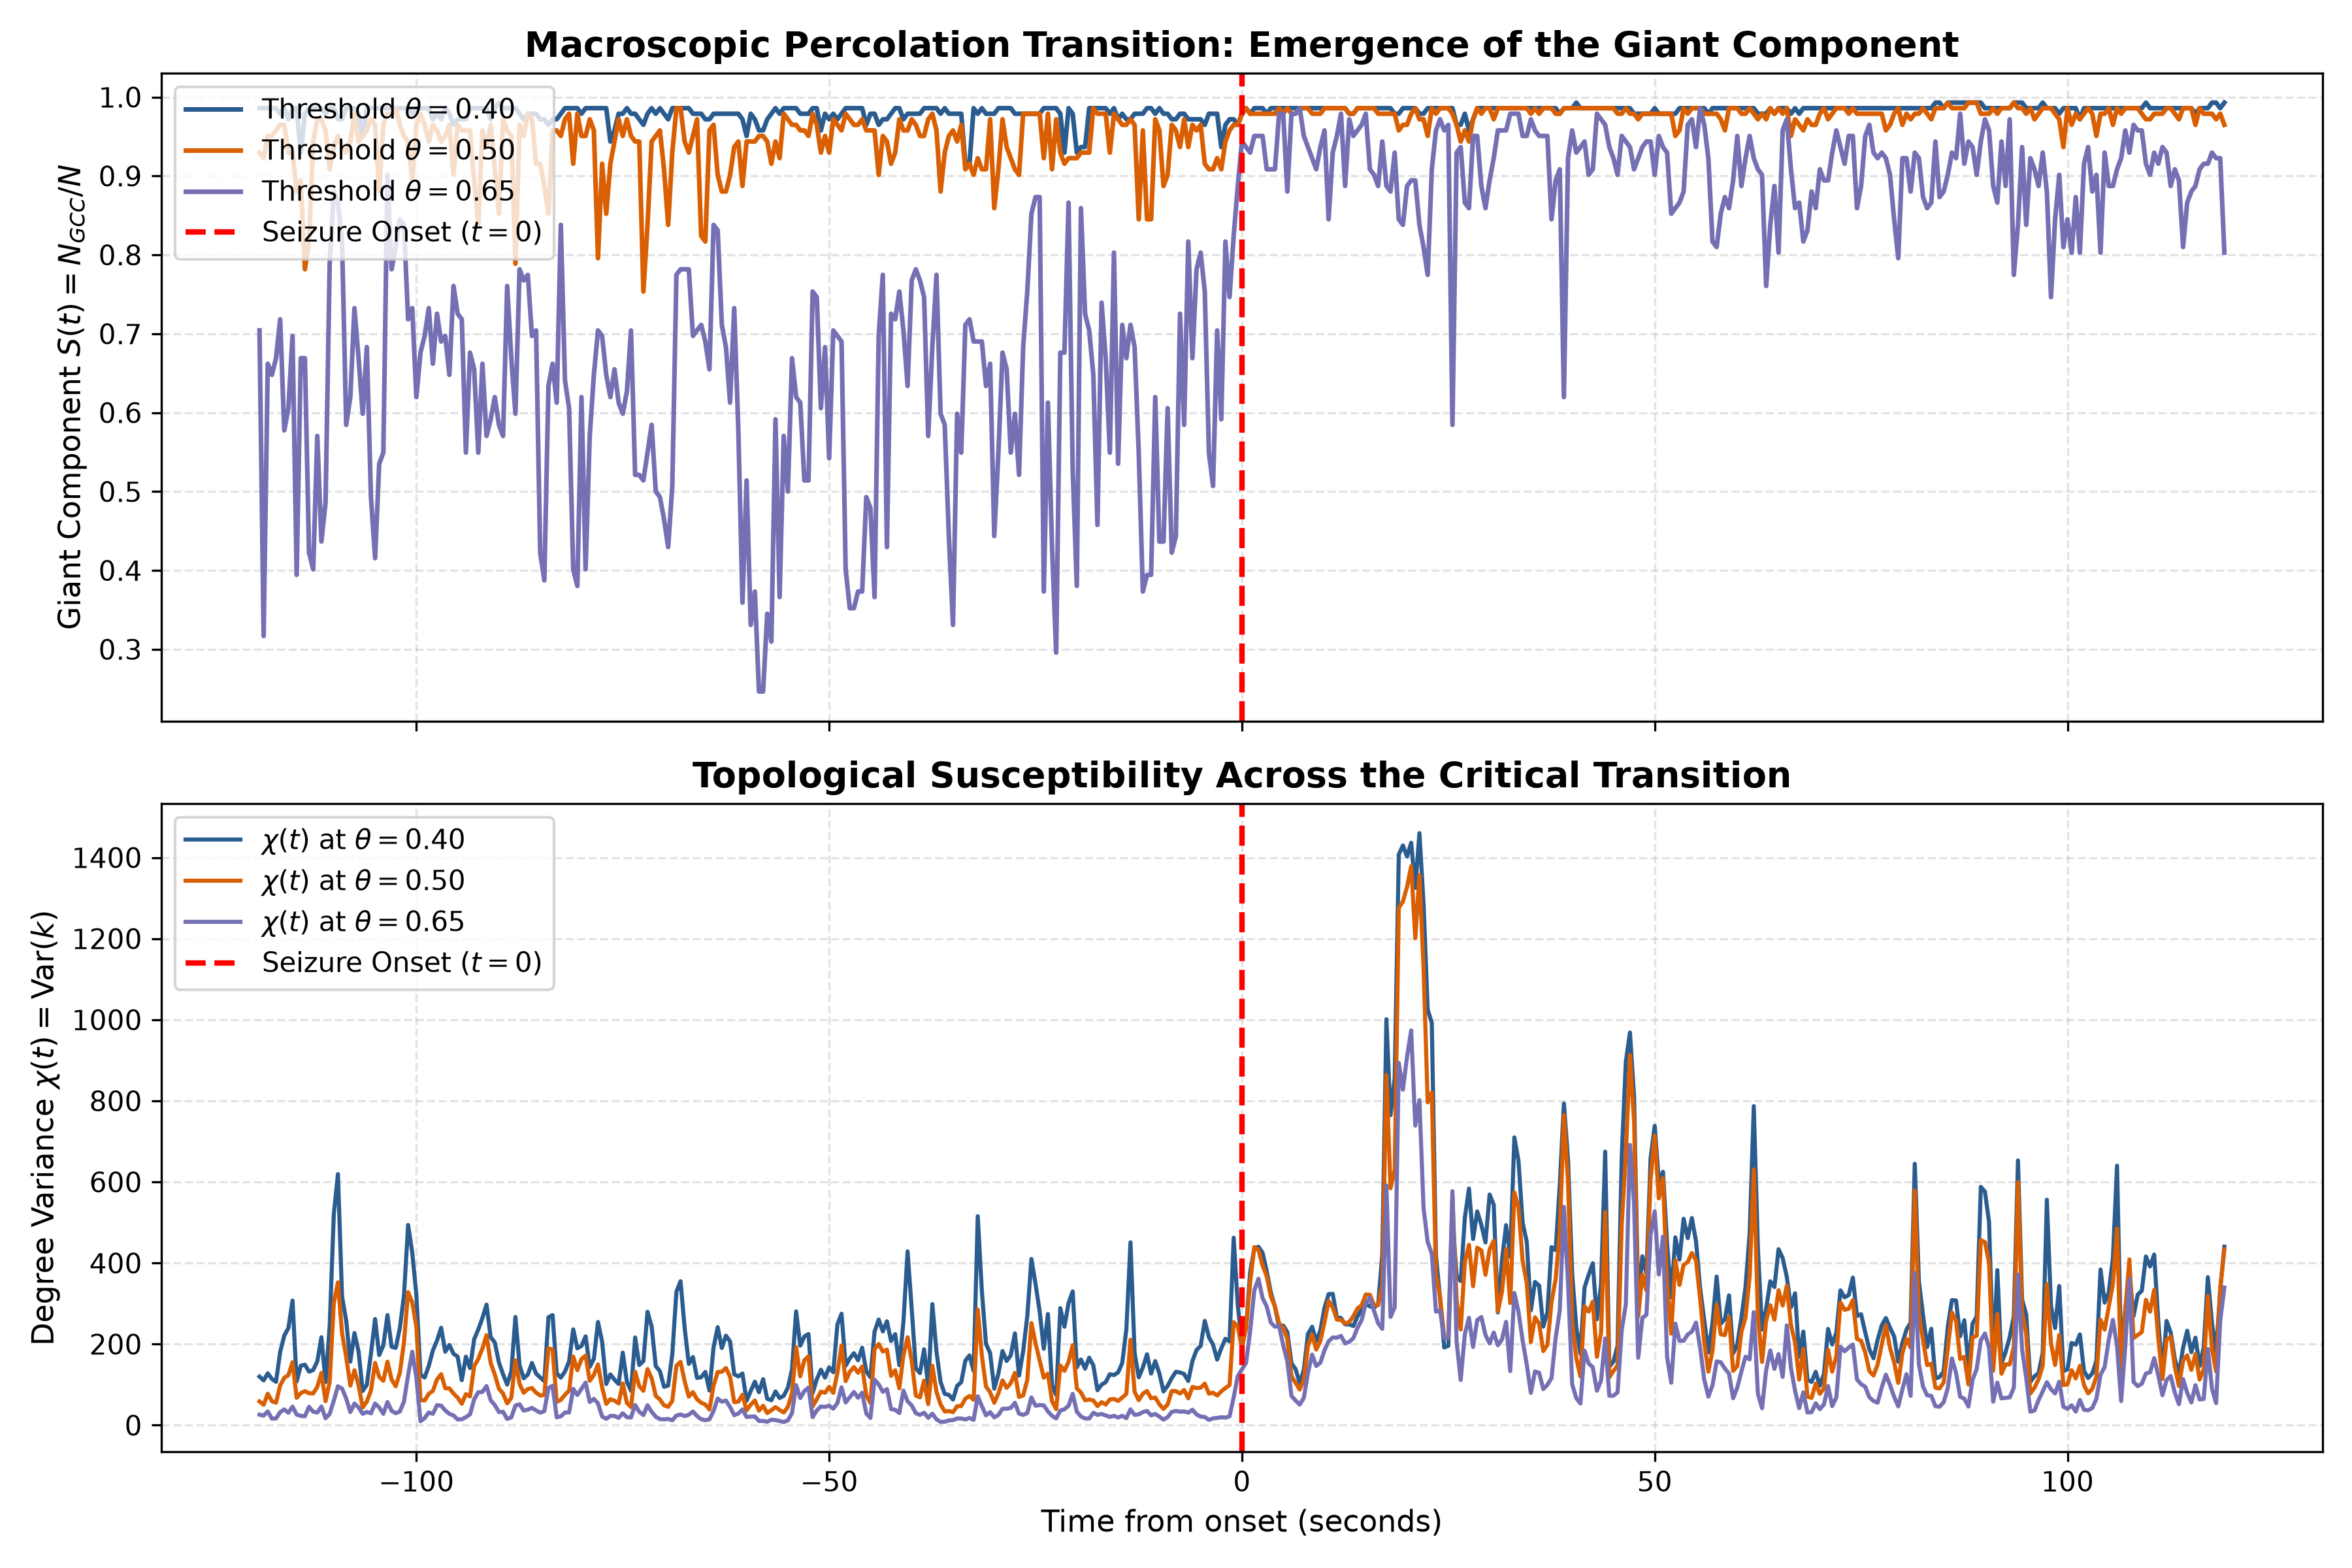
\includegraphics[width=0.8\textwidth]{img/DQ0040P6/macro_percolation_transition.png}
    \caption{Macroscopic Percolation ($S(\tau)$ and $\chi(\tau)$) for recording \texttt{DQ0040P6}.}
    \label{fig:dq0040p6_macro}
\end{figure}

\begin{figure}[htbp]
    \centering
    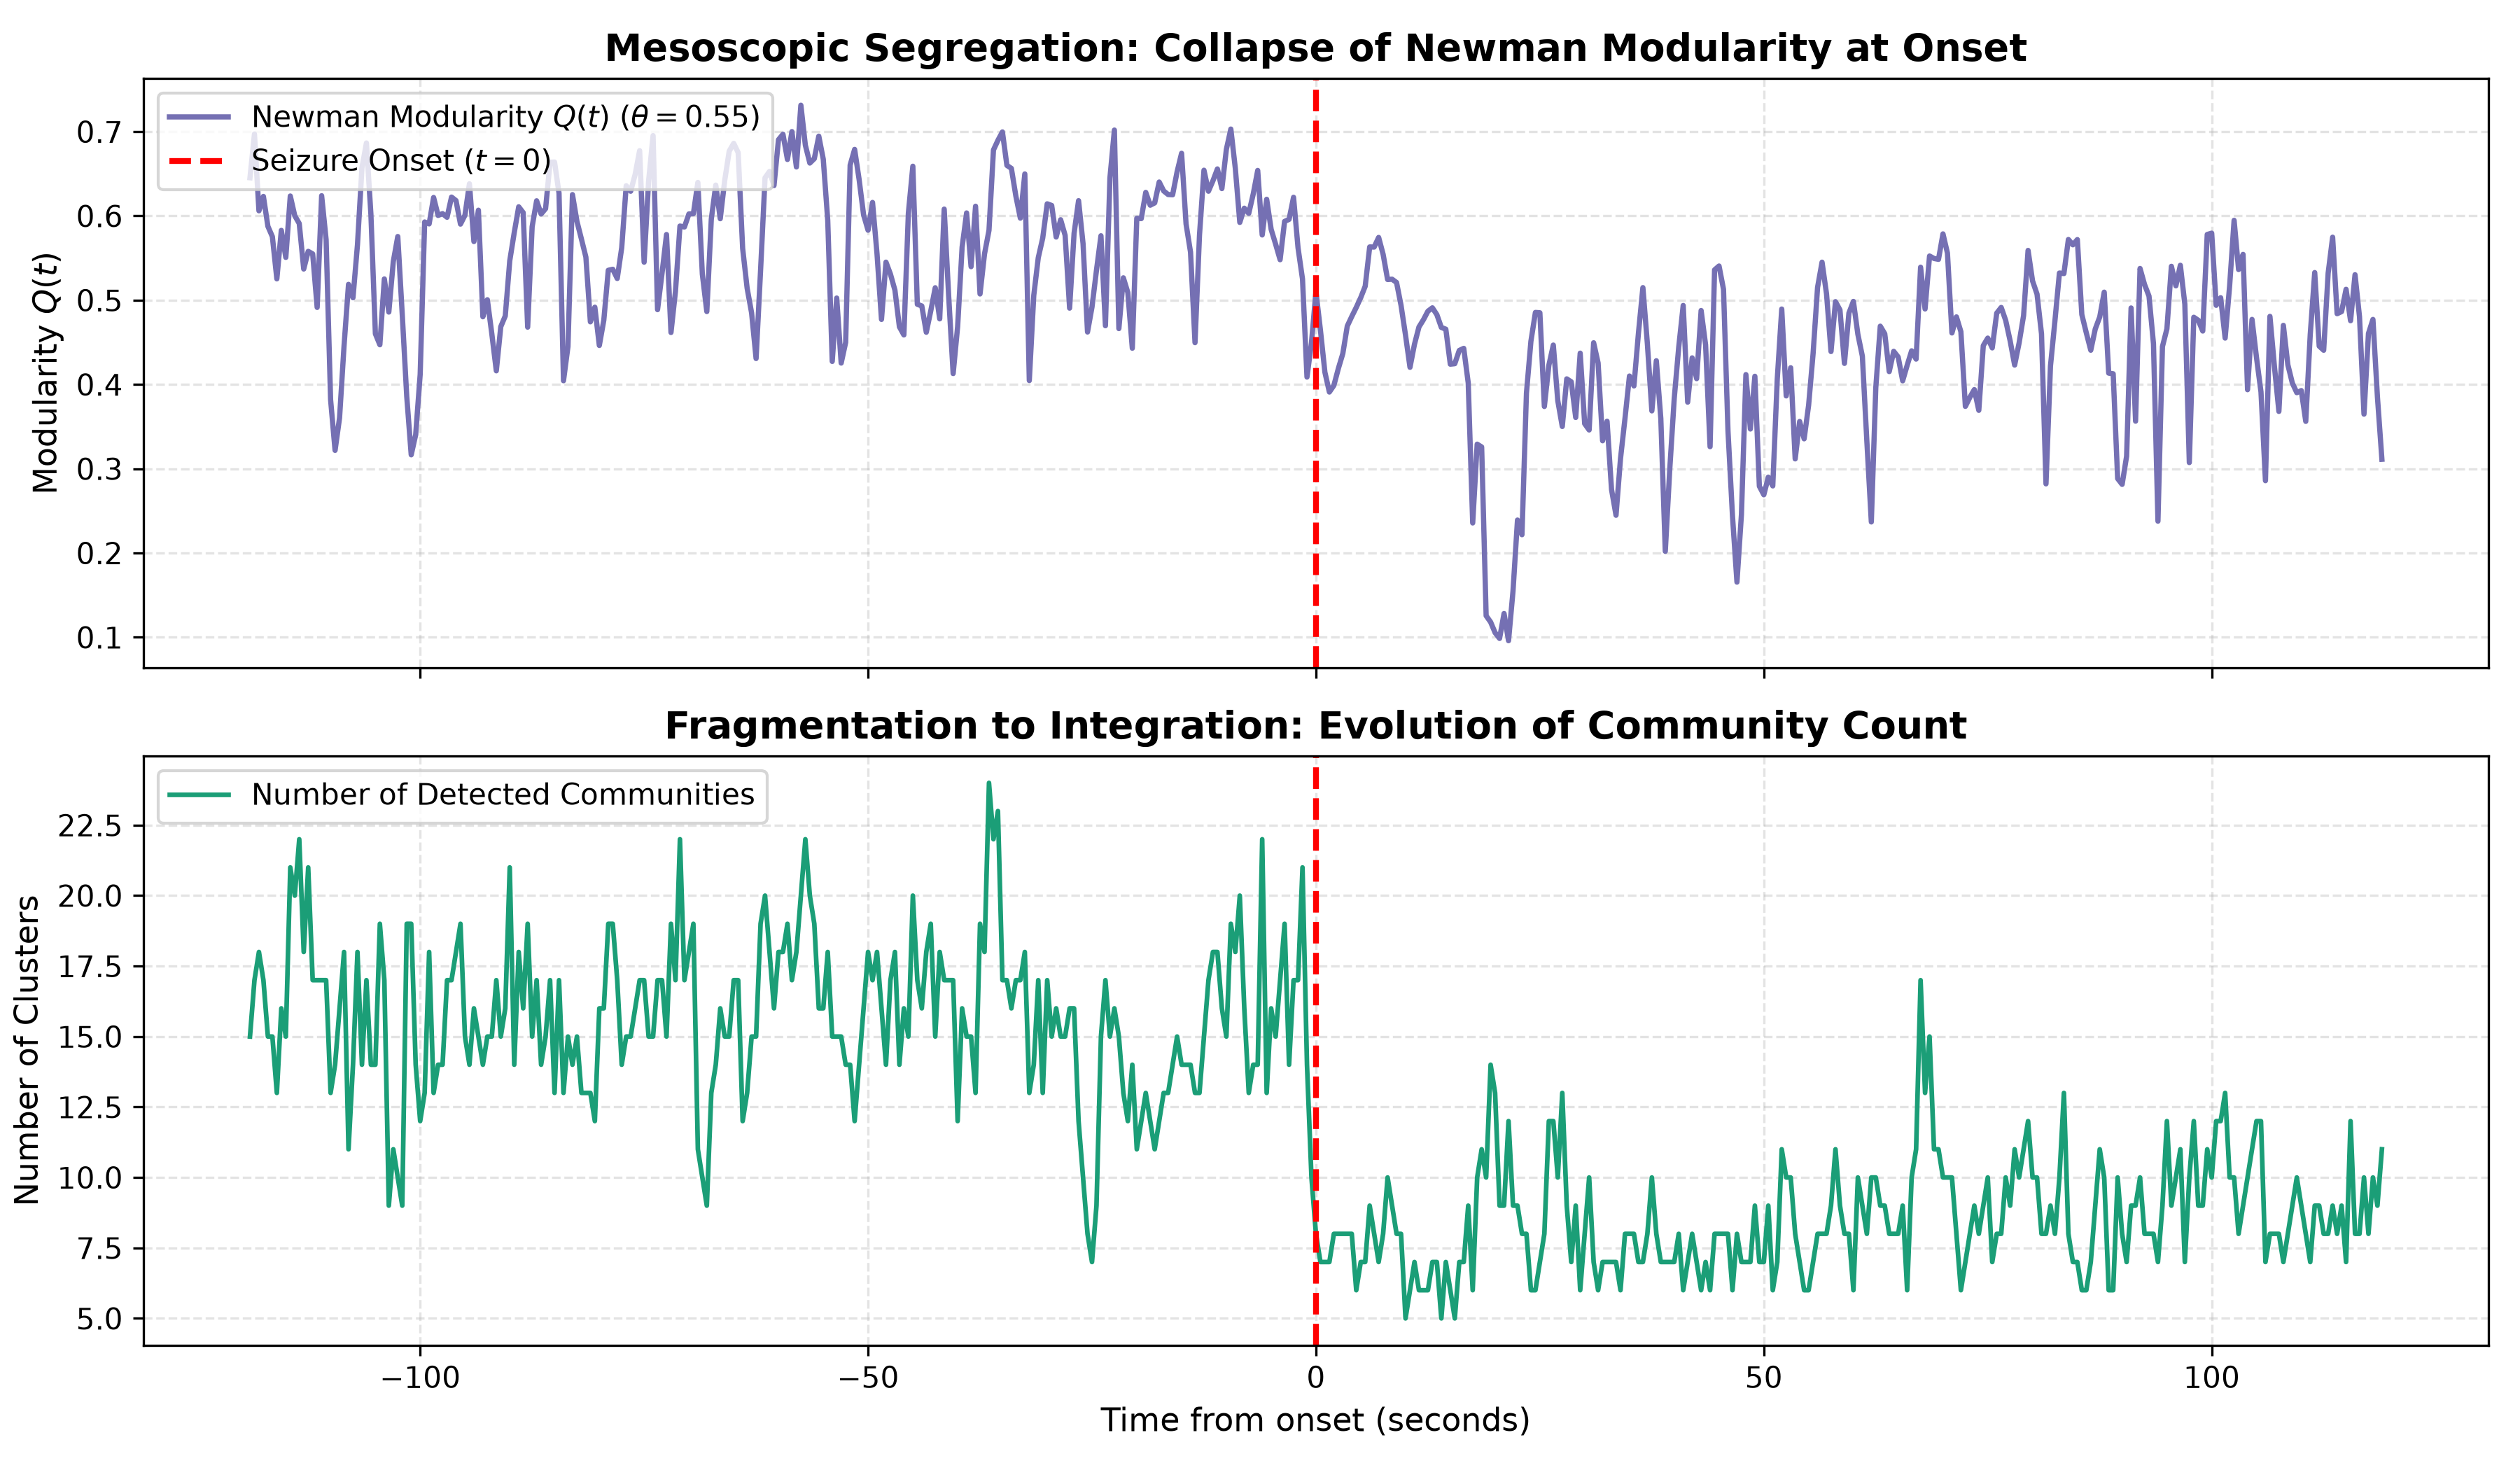
\includegraphics[width=0.8\textwidth]{img/DQ0040P6/meso_modularity_collapse.png}
    \caption{Mesoscopic Modularity Collapse ($Q(\tau)$ and $N_c(\tau)$) for recording \texttt{DQ0040P6}.}
    \label{fig:dq0040p6_meso}
\end{figure}

\begin{figure}[htbp]
    \centering
    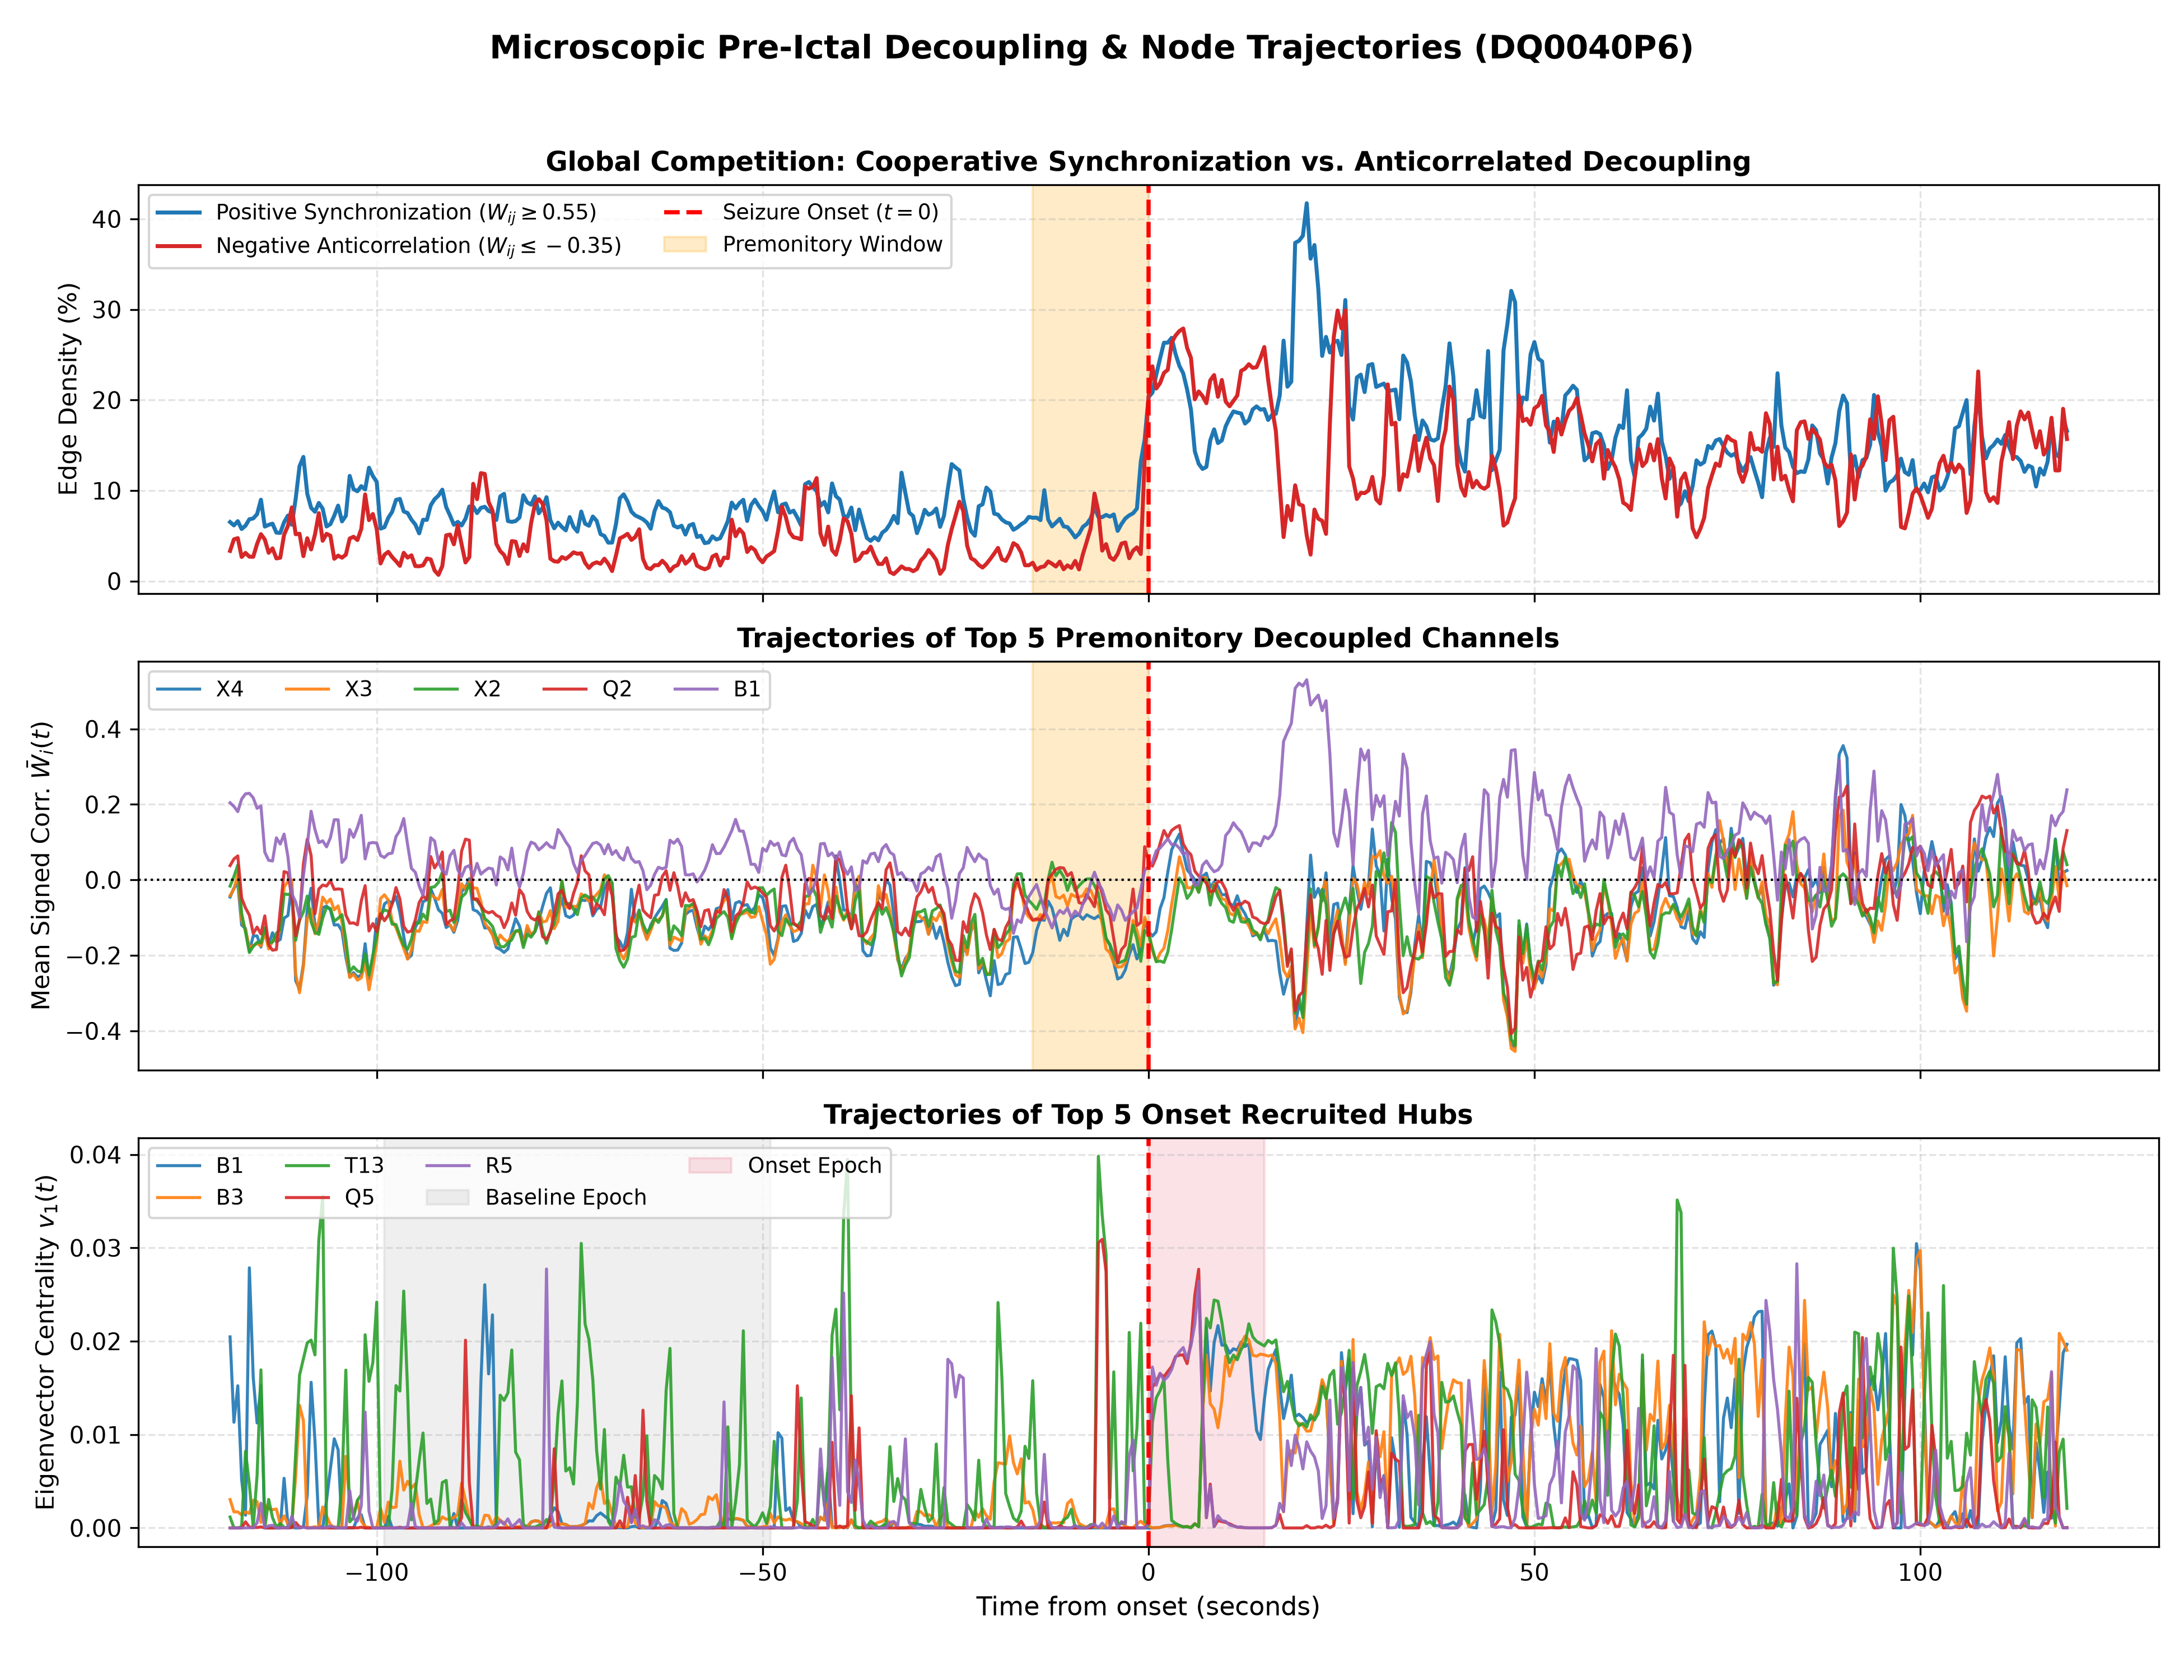
\includegraphics[width=0.8\textwidth]{img/DQ0040P6/micro_premonitory_decoupling.png}
    \caption{Premonitory Decoupling and Hub Trajectories for recording \texttt{DQ0040P6}.}
    \label{fig:dq0040p6_micro_traj}
\end{figure}

\begin{figure}[htbp]
    \centering
    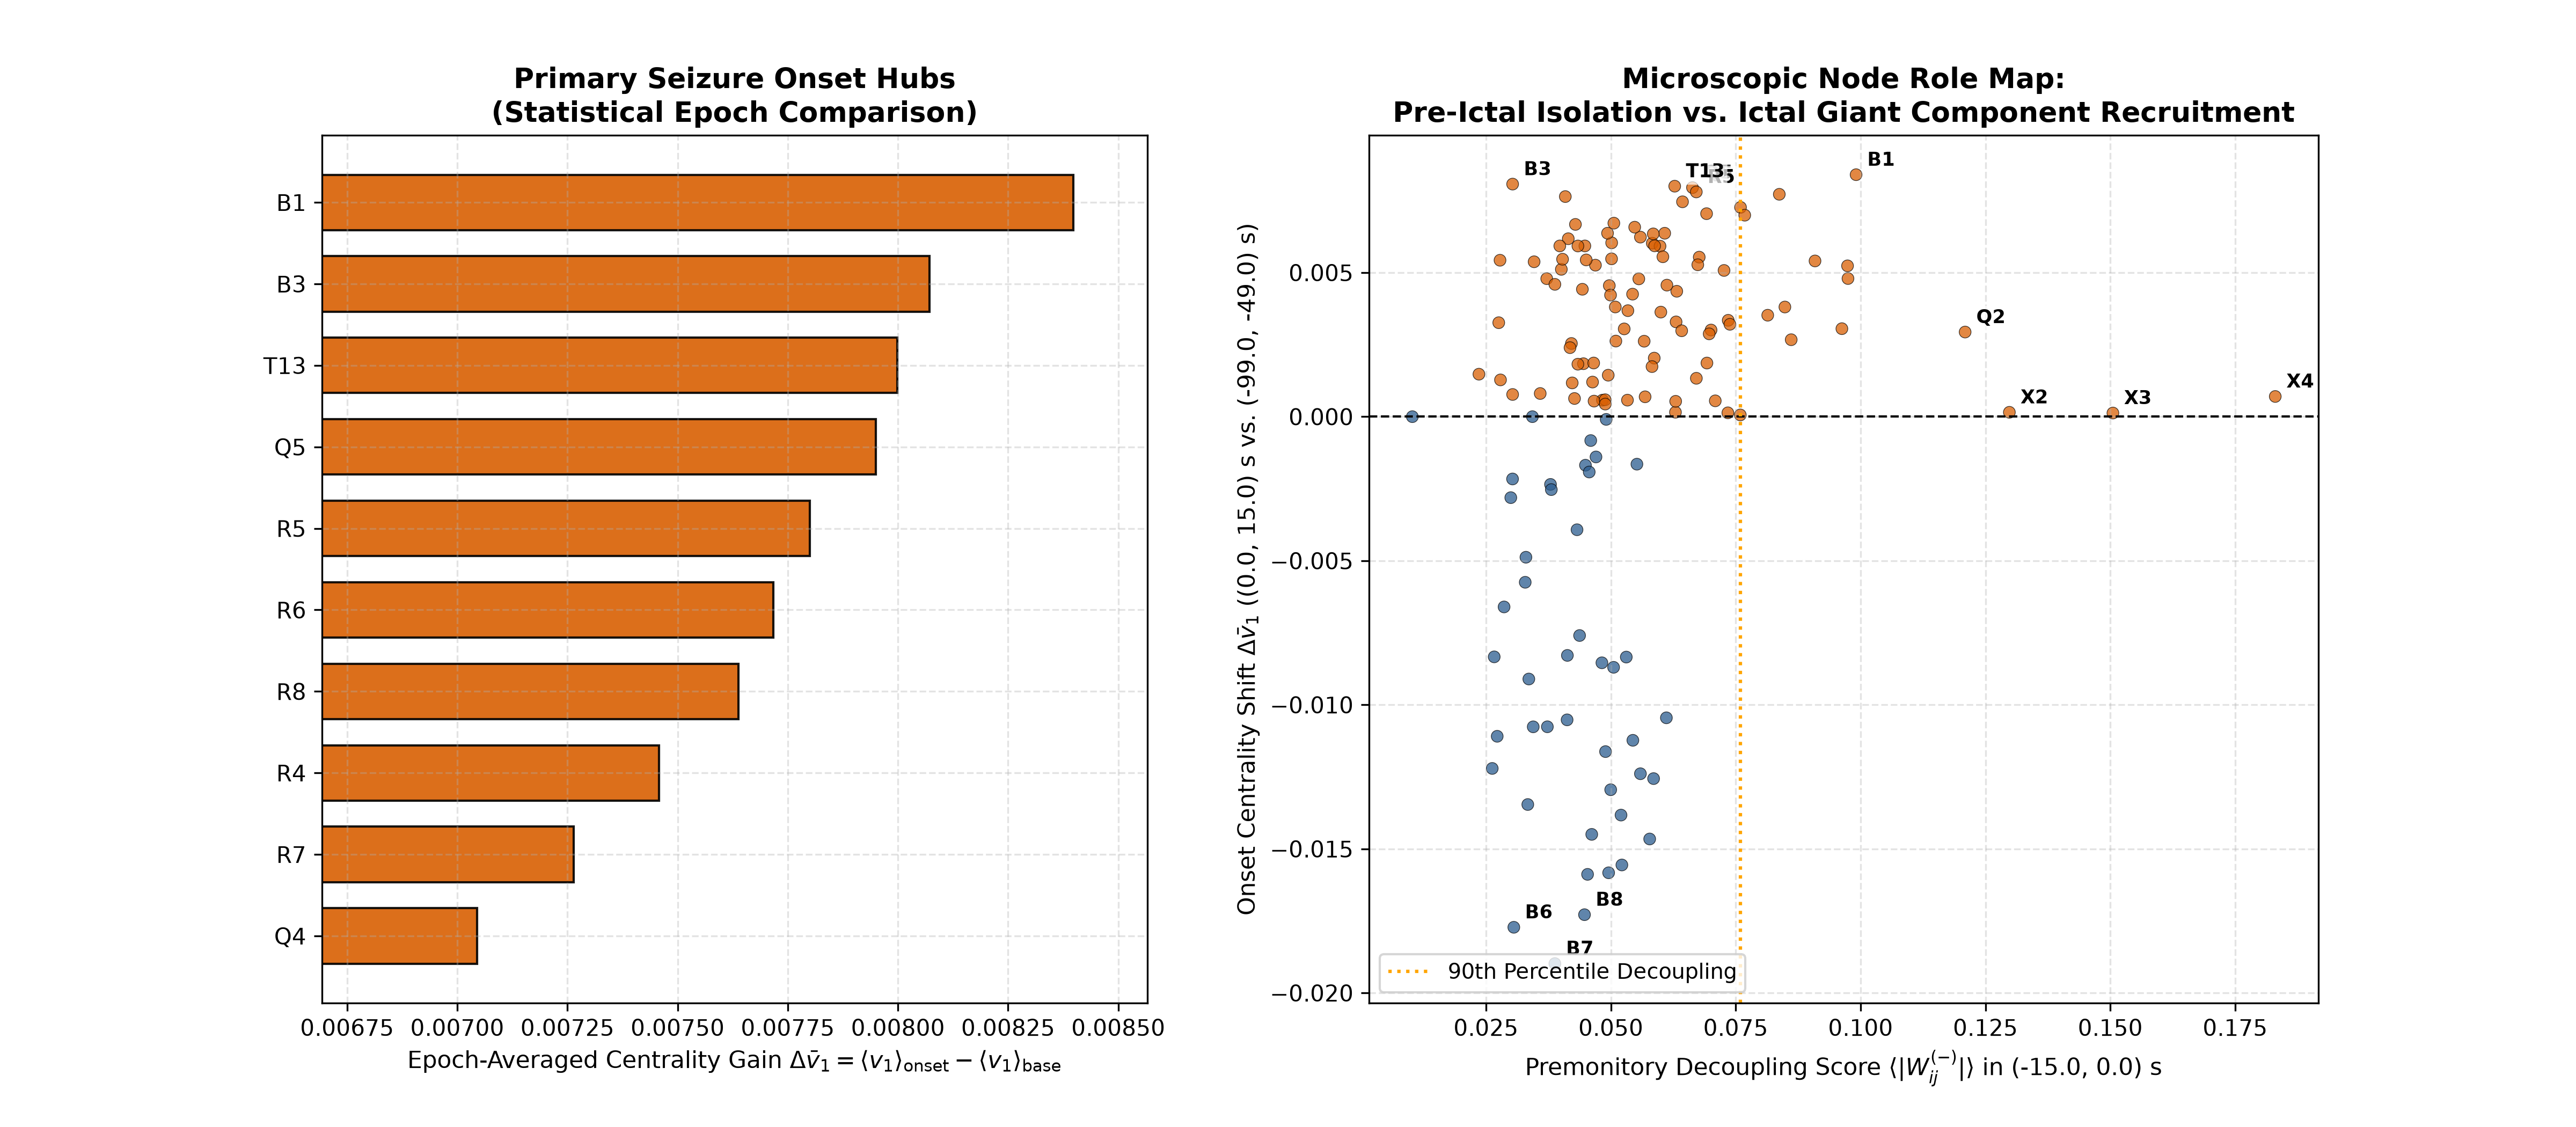
\includegraphics[width=0.9\textwidth]{img/DQ0040P6/micro_hub_recruitment_and_roles.png}
    \caption{Onset Hub Ranking and 2D Functional Role Map for recording \texttt{DQ0040P6}.}
    \label{fig:dq0040p6_micro_roles}
\end{figure}

\clearpage

\subsection{Recording \texttt{DQ0040WG}}
\label{app:rec_dq0040wg}

\begin{figure}[htbp]
    \centering
    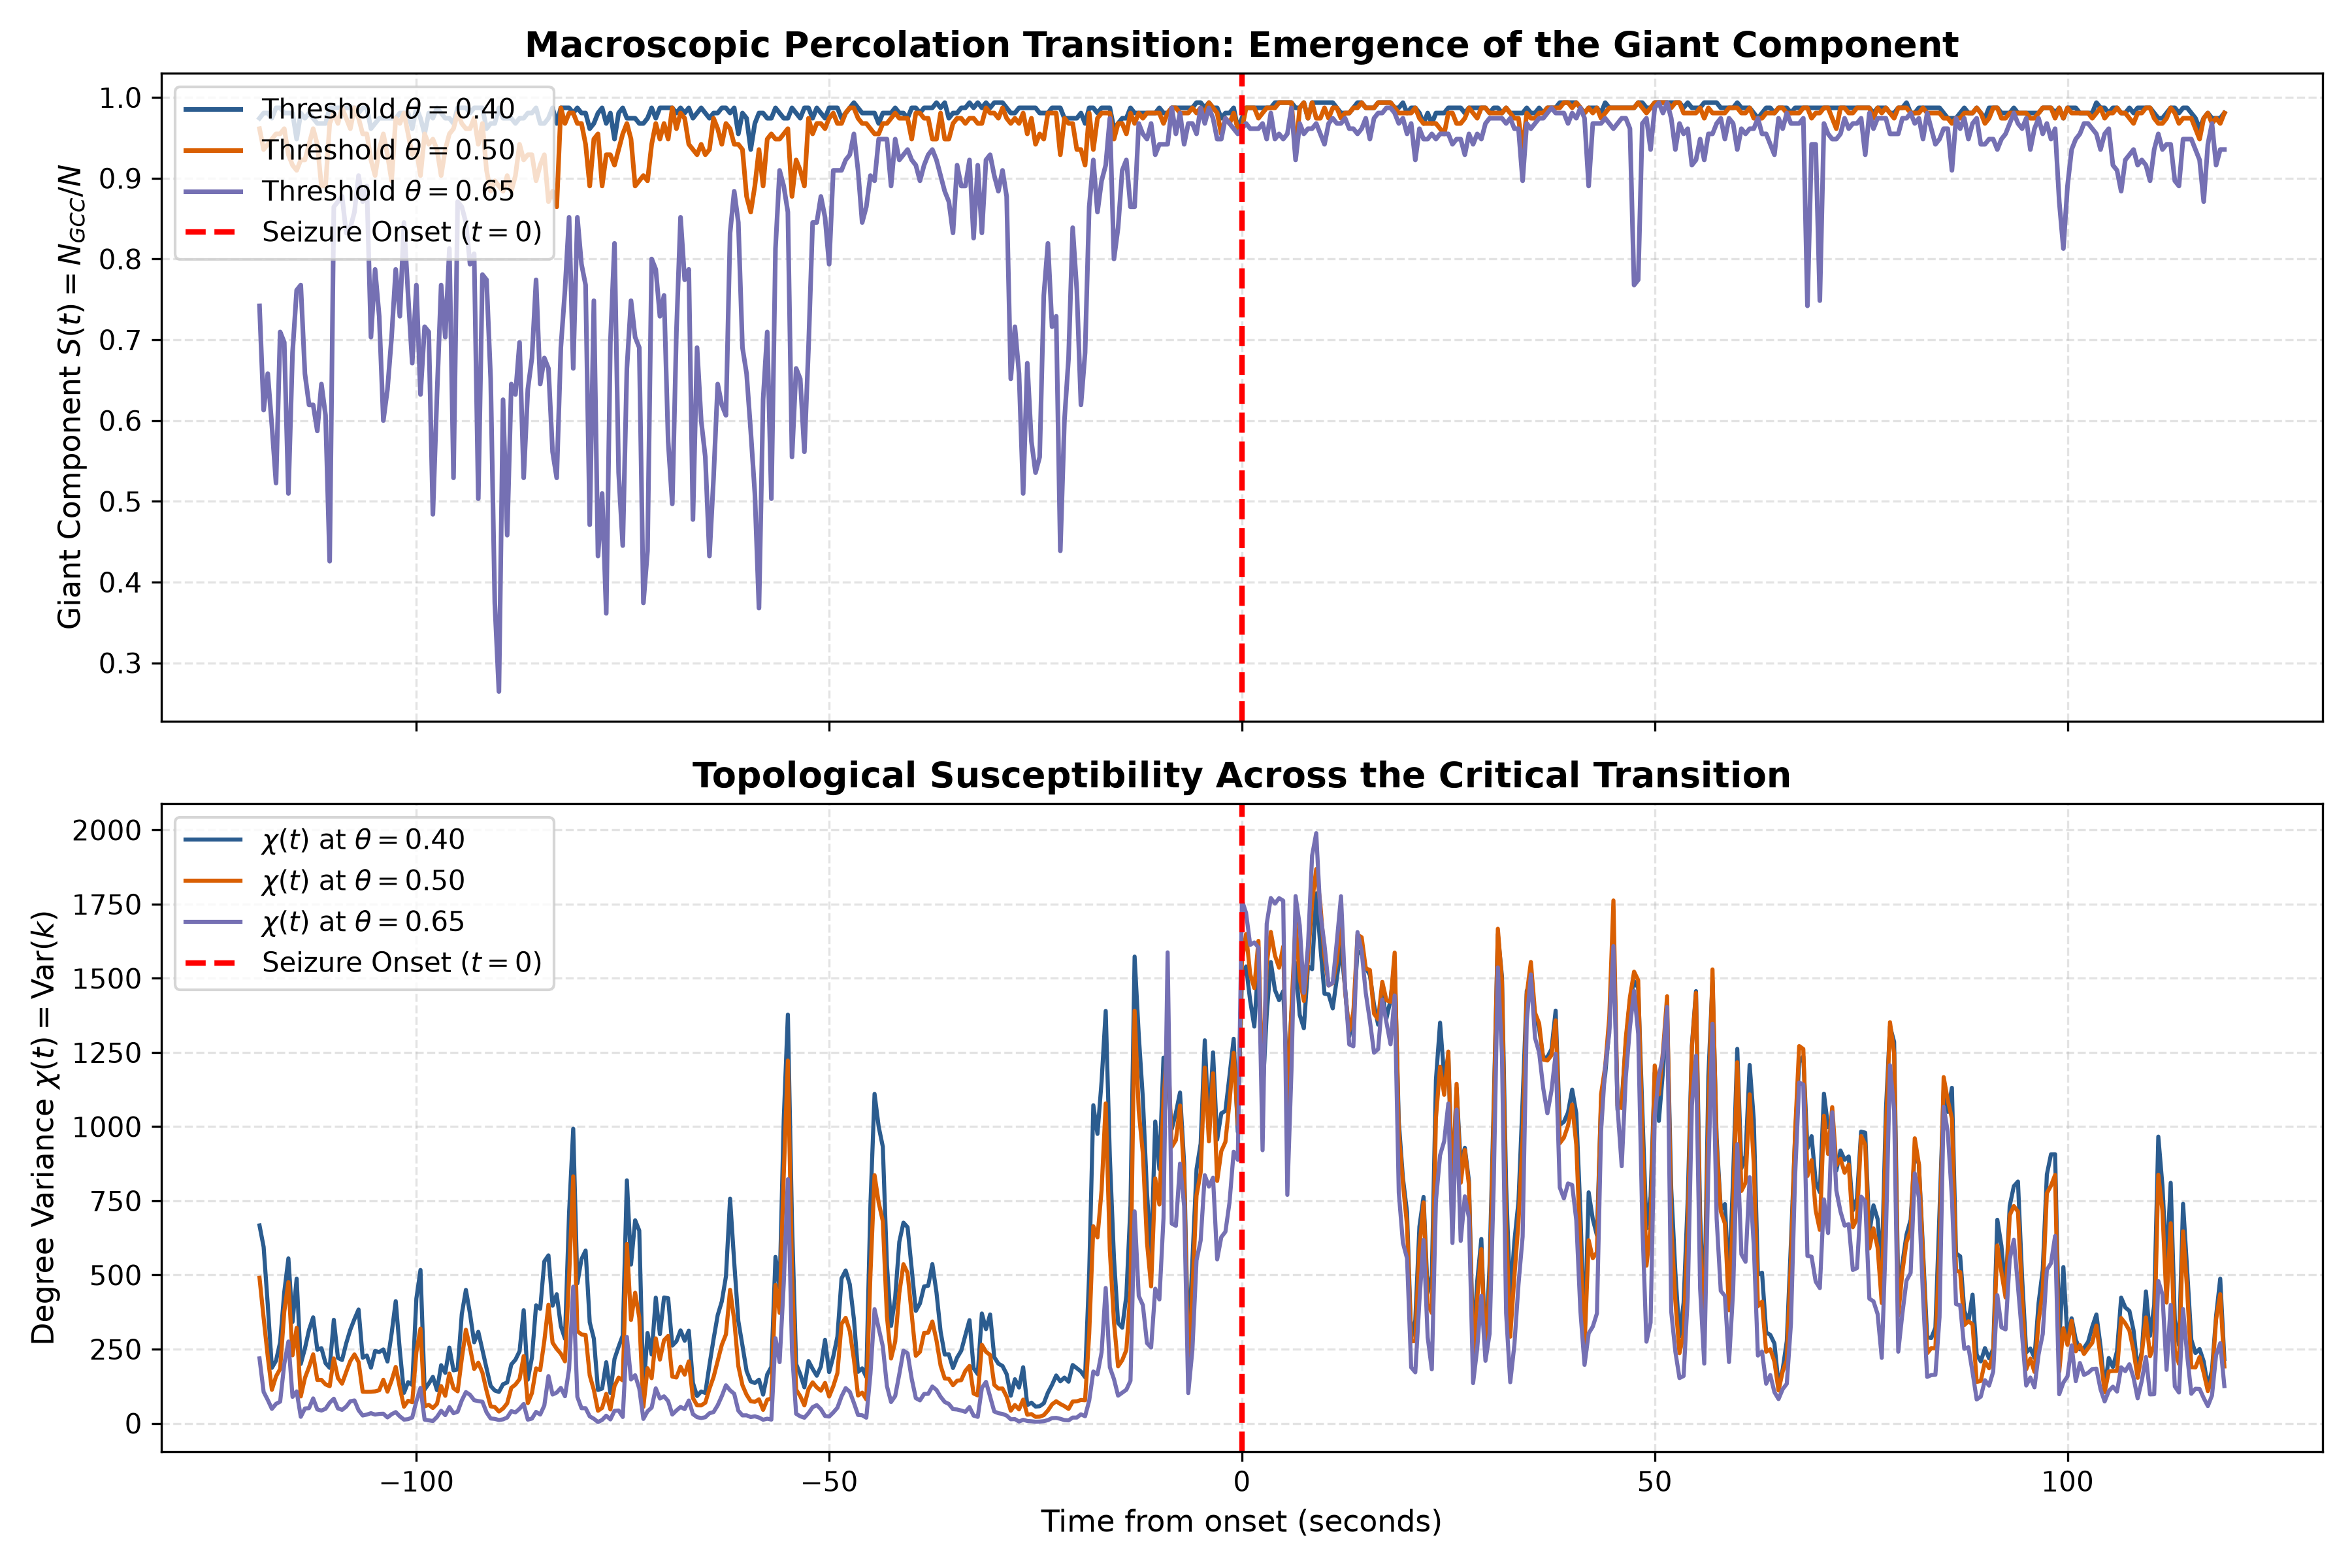
\includegraphics[width=0.8\textwidth]{img/DQ0040WG/macro_percolation_transition.png}
    \caption{Macroscopic Percolation ($S(\tau)$ and $\chi(\tau)$) for recording \texttt{DQ0040WG}.}
    \label{fig:dq0040wg_macro}
\end{figure}

\begin{figure}[htbp]
    \centering
    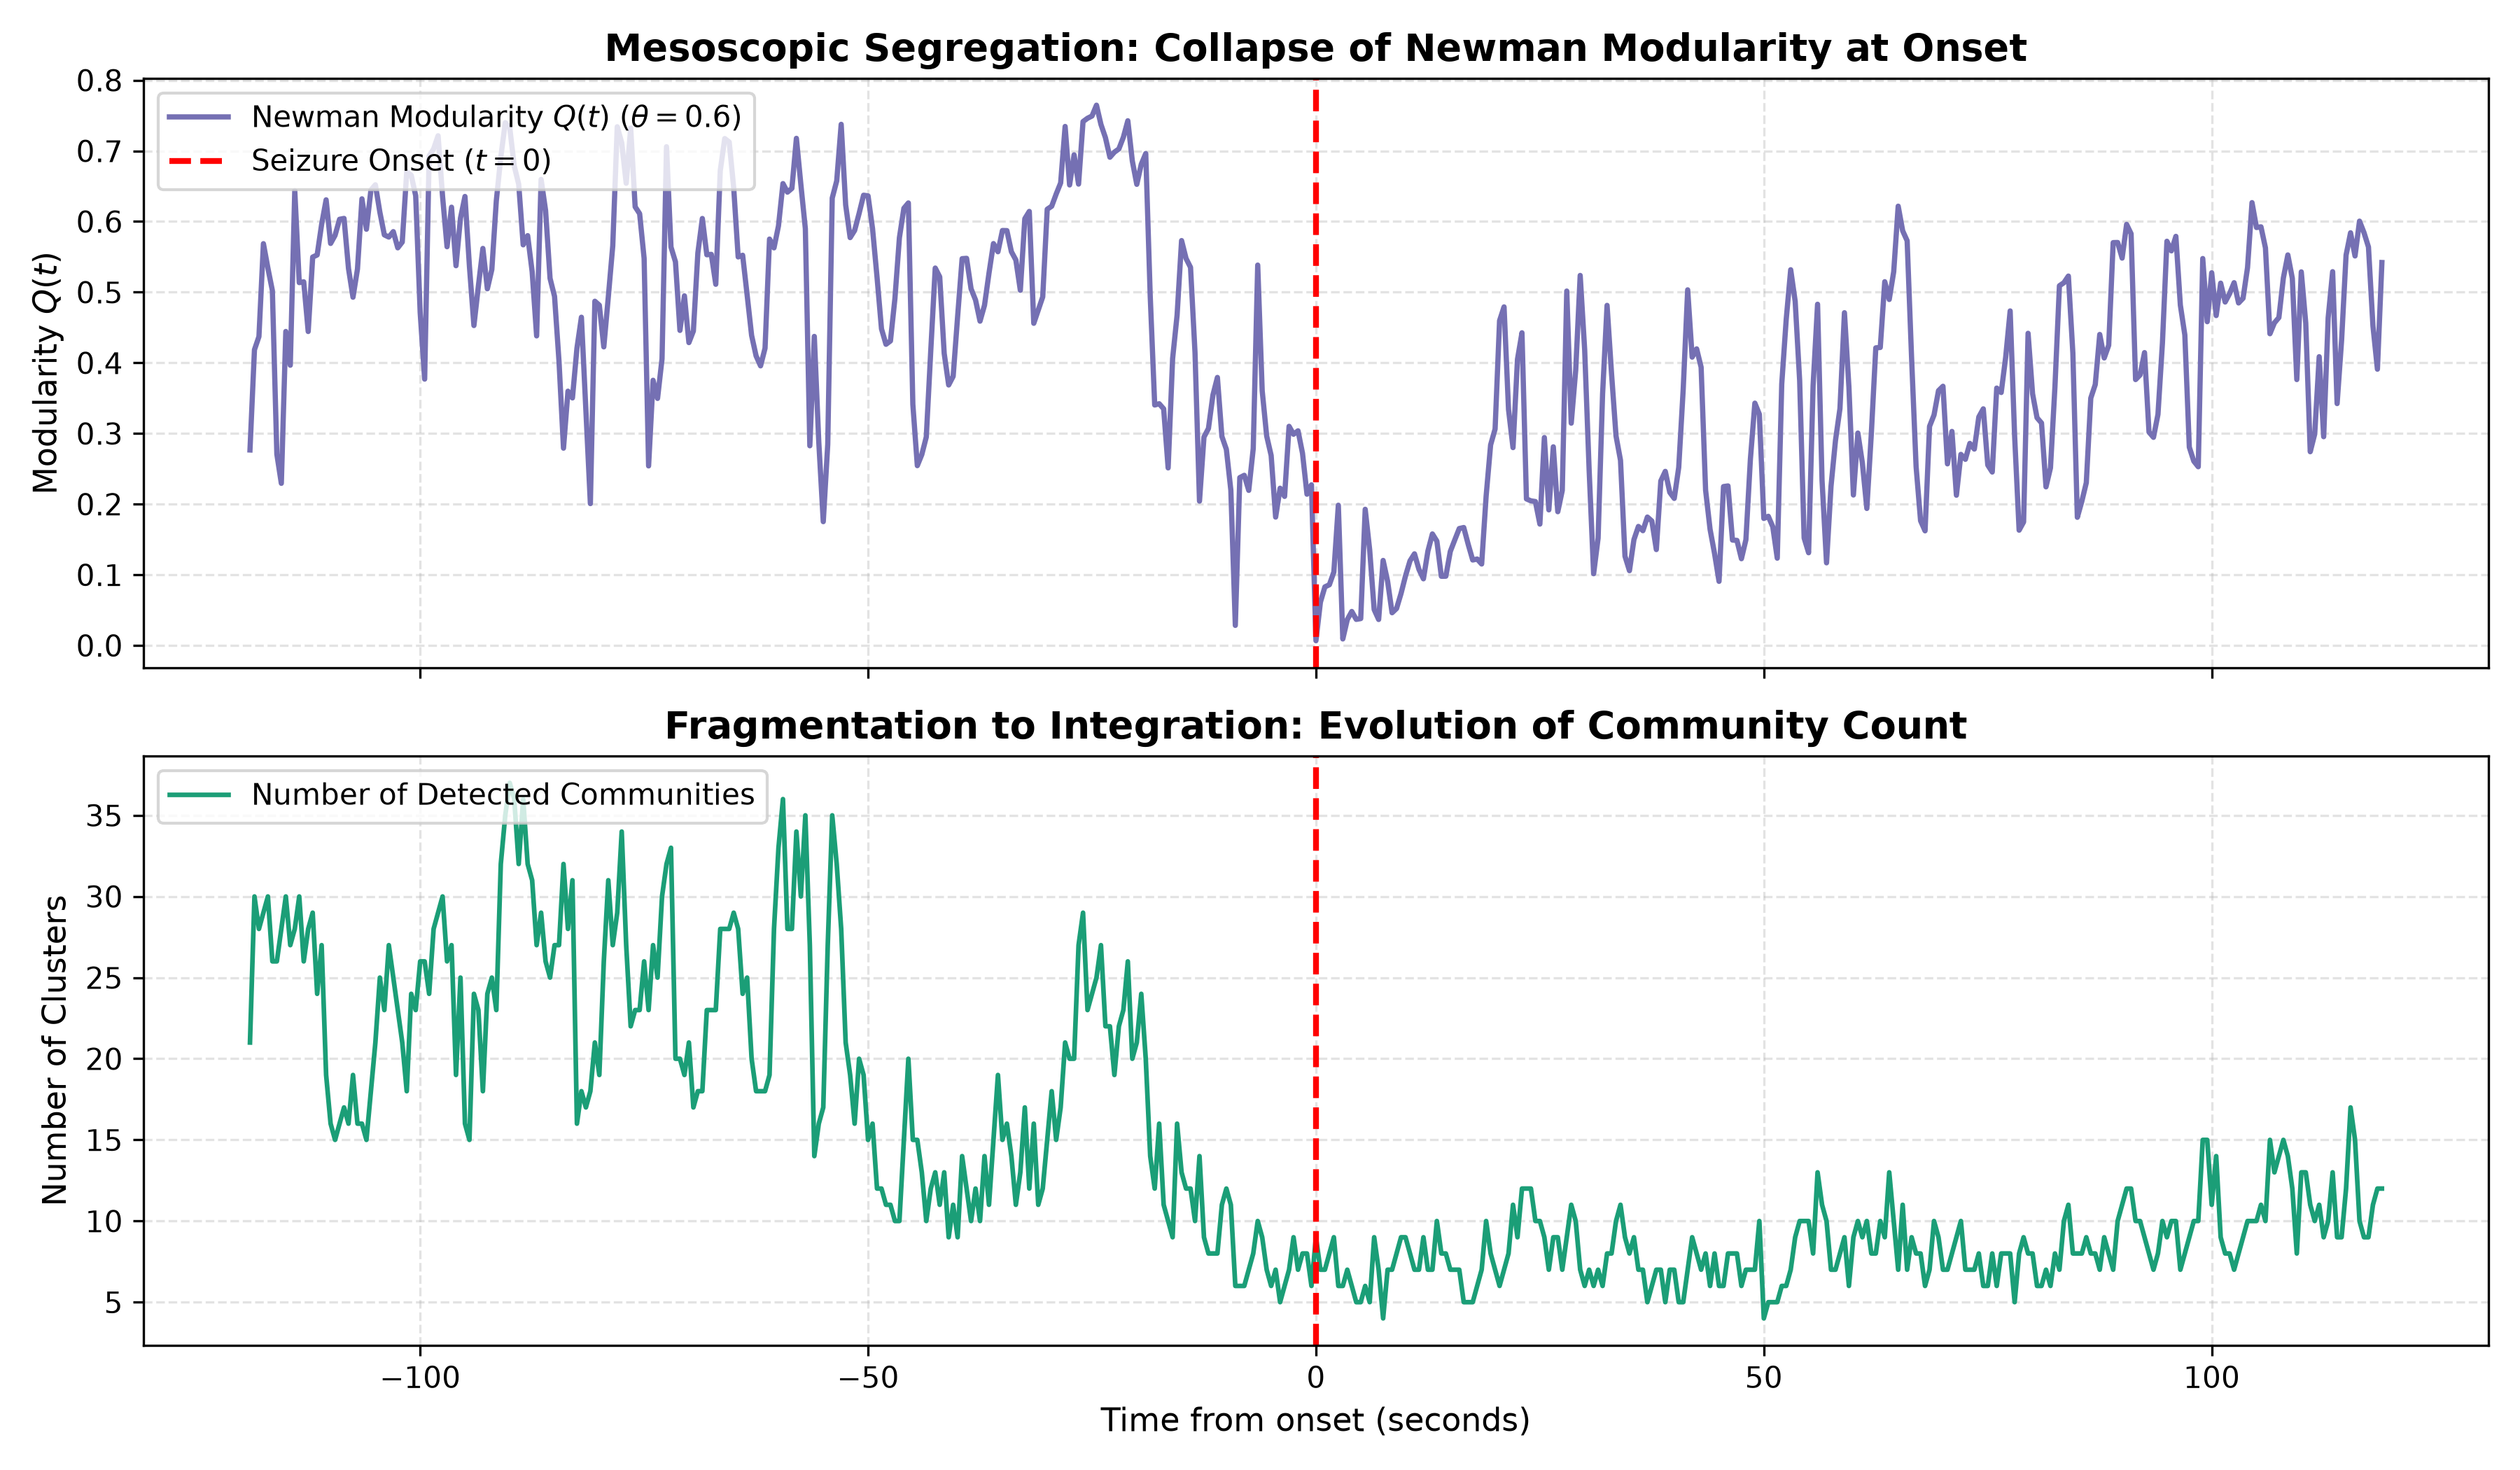
\includegraphics[width=0.8\textwidth]{img/DQ0040WG/meso_modularity_collapse.png}
    \caption{Mesoscopic Modularity Collapse ($Q(\tau)$ and $N_c(\tau)$) for recording \texttt{DQ0040WG}.}
    \label{fig:dq0040wg_meso}
\end{figure}

\begin{figure}[htbp]
    \centering
    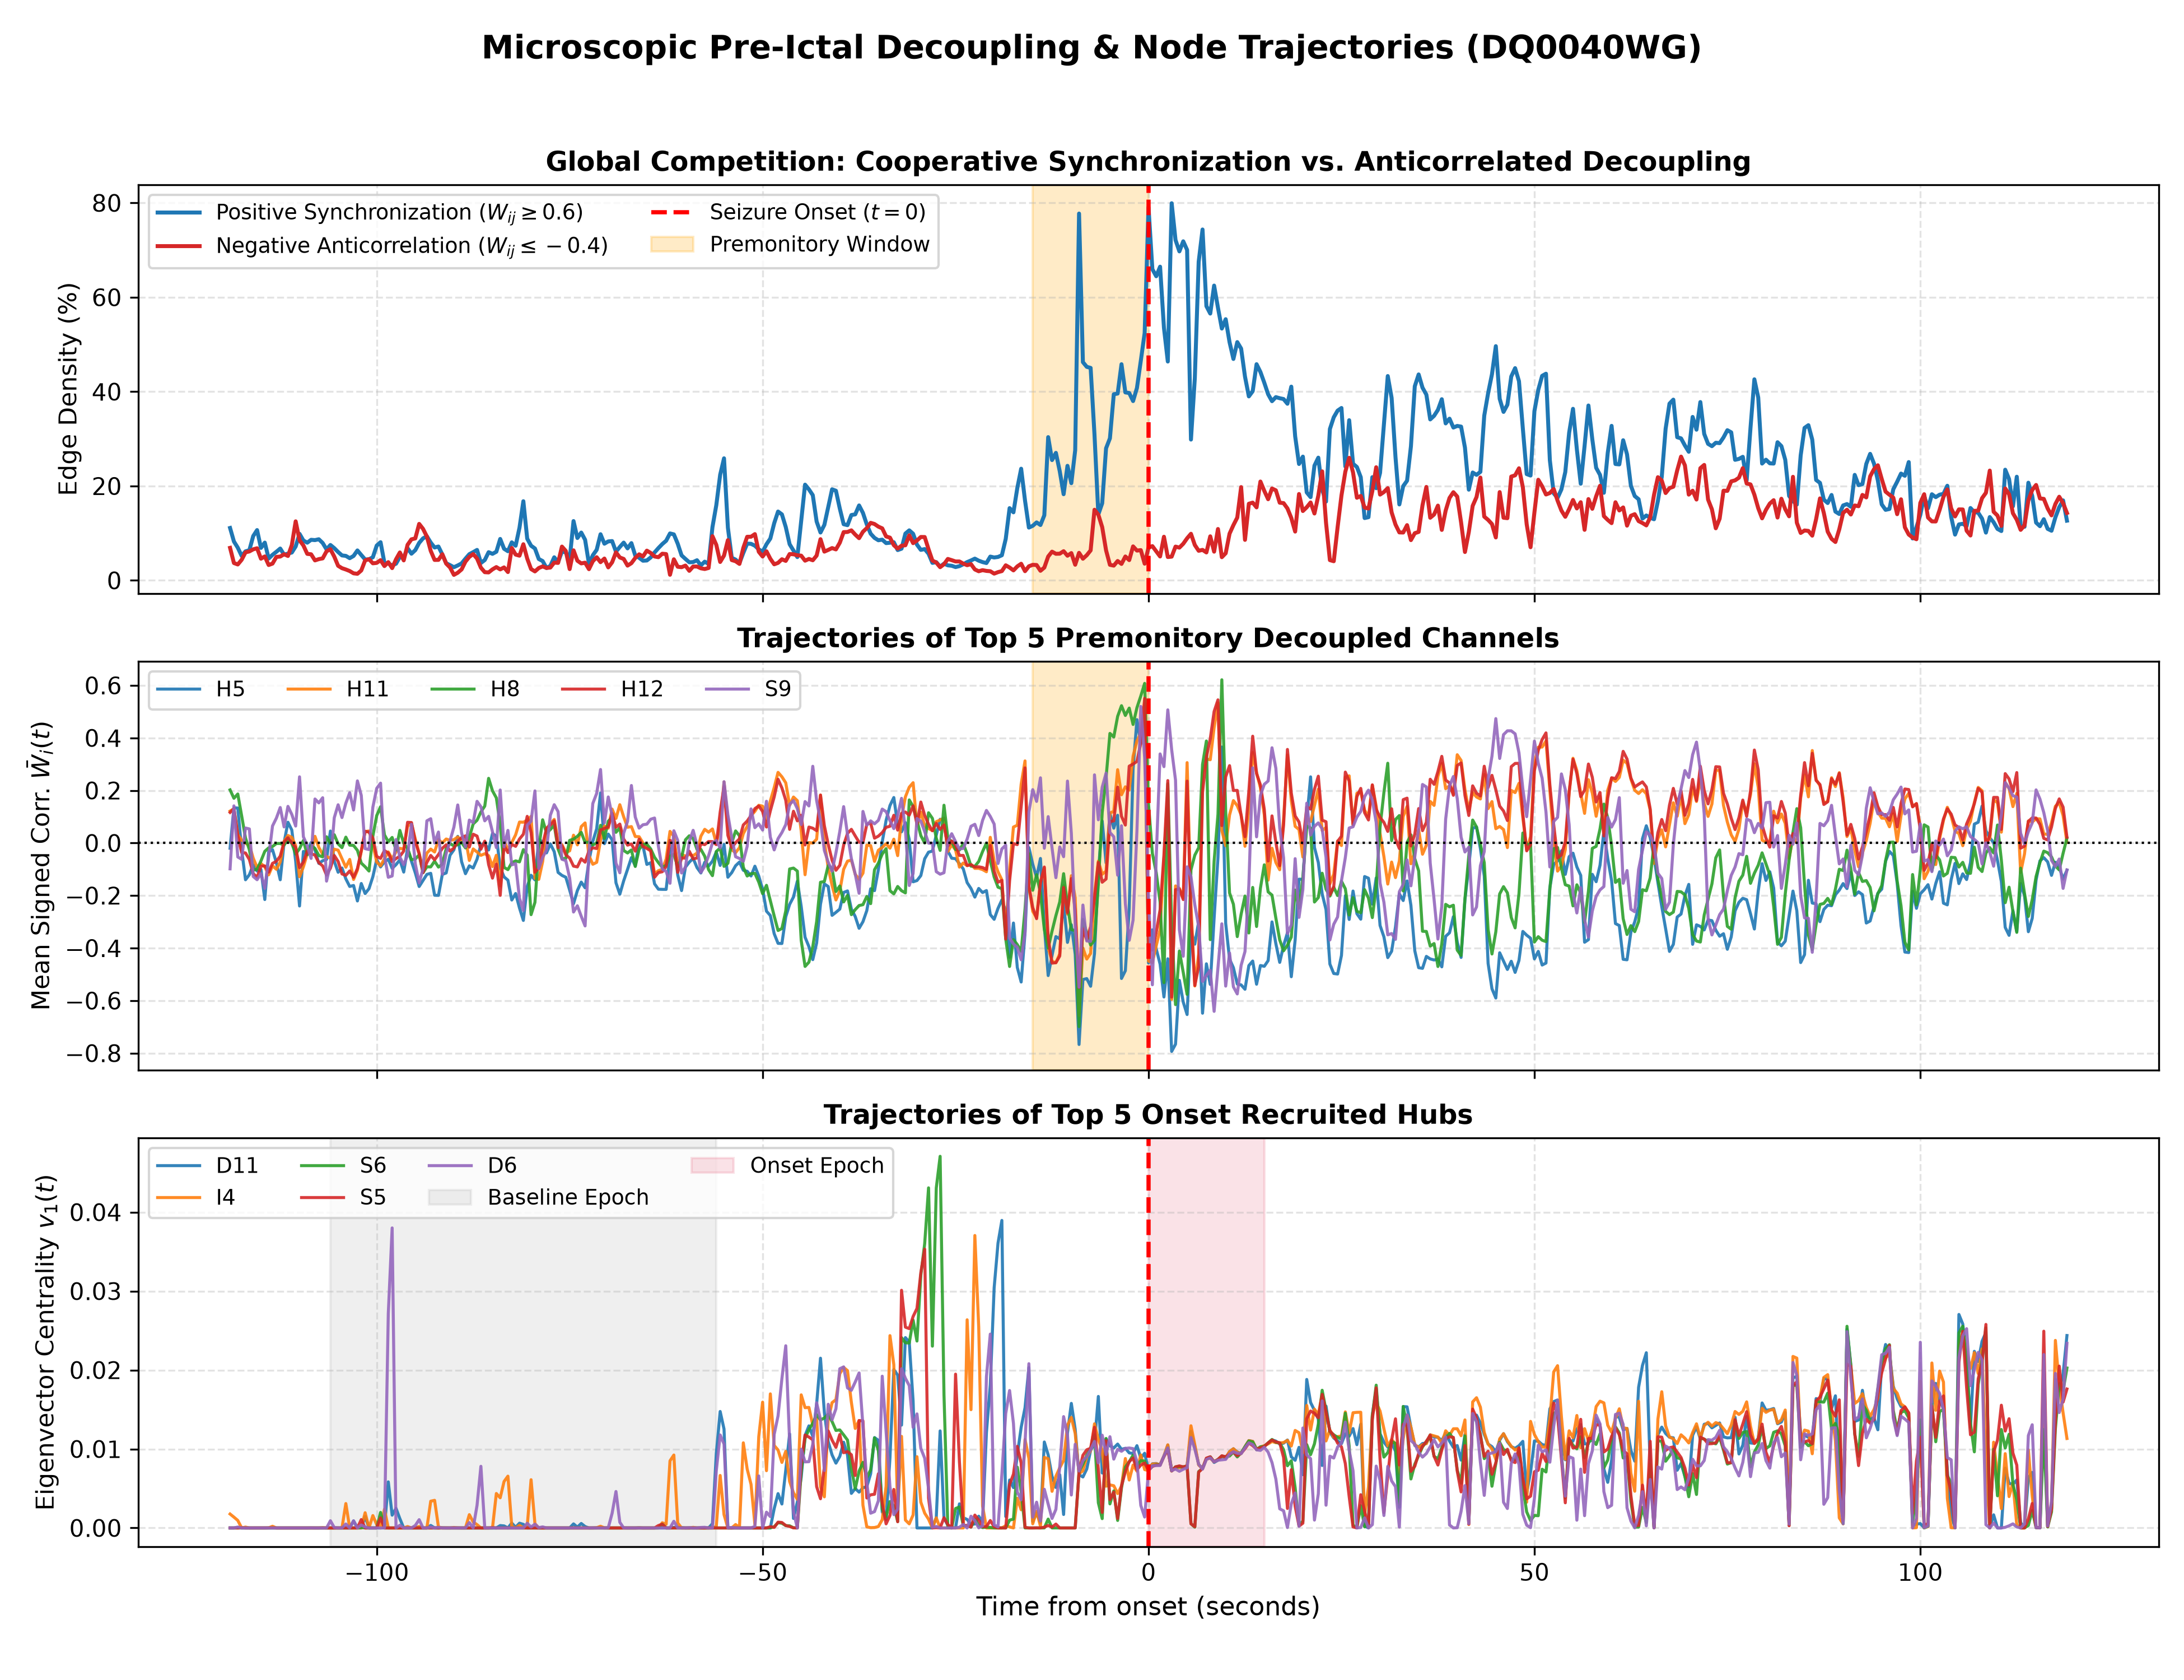
\includegraphics[width=0.8\textwidth]{img/DQ0040WG/micro_premonitory_decoupling.png}
    \caption{Premonitory Decoupling and Hub Trajectories for recording \texttt{DQ0040WG}.}
    \label{fig:dq0040wg_micro_traj}
\end{figure}

\begin{figure}[htbp]
    \centering
    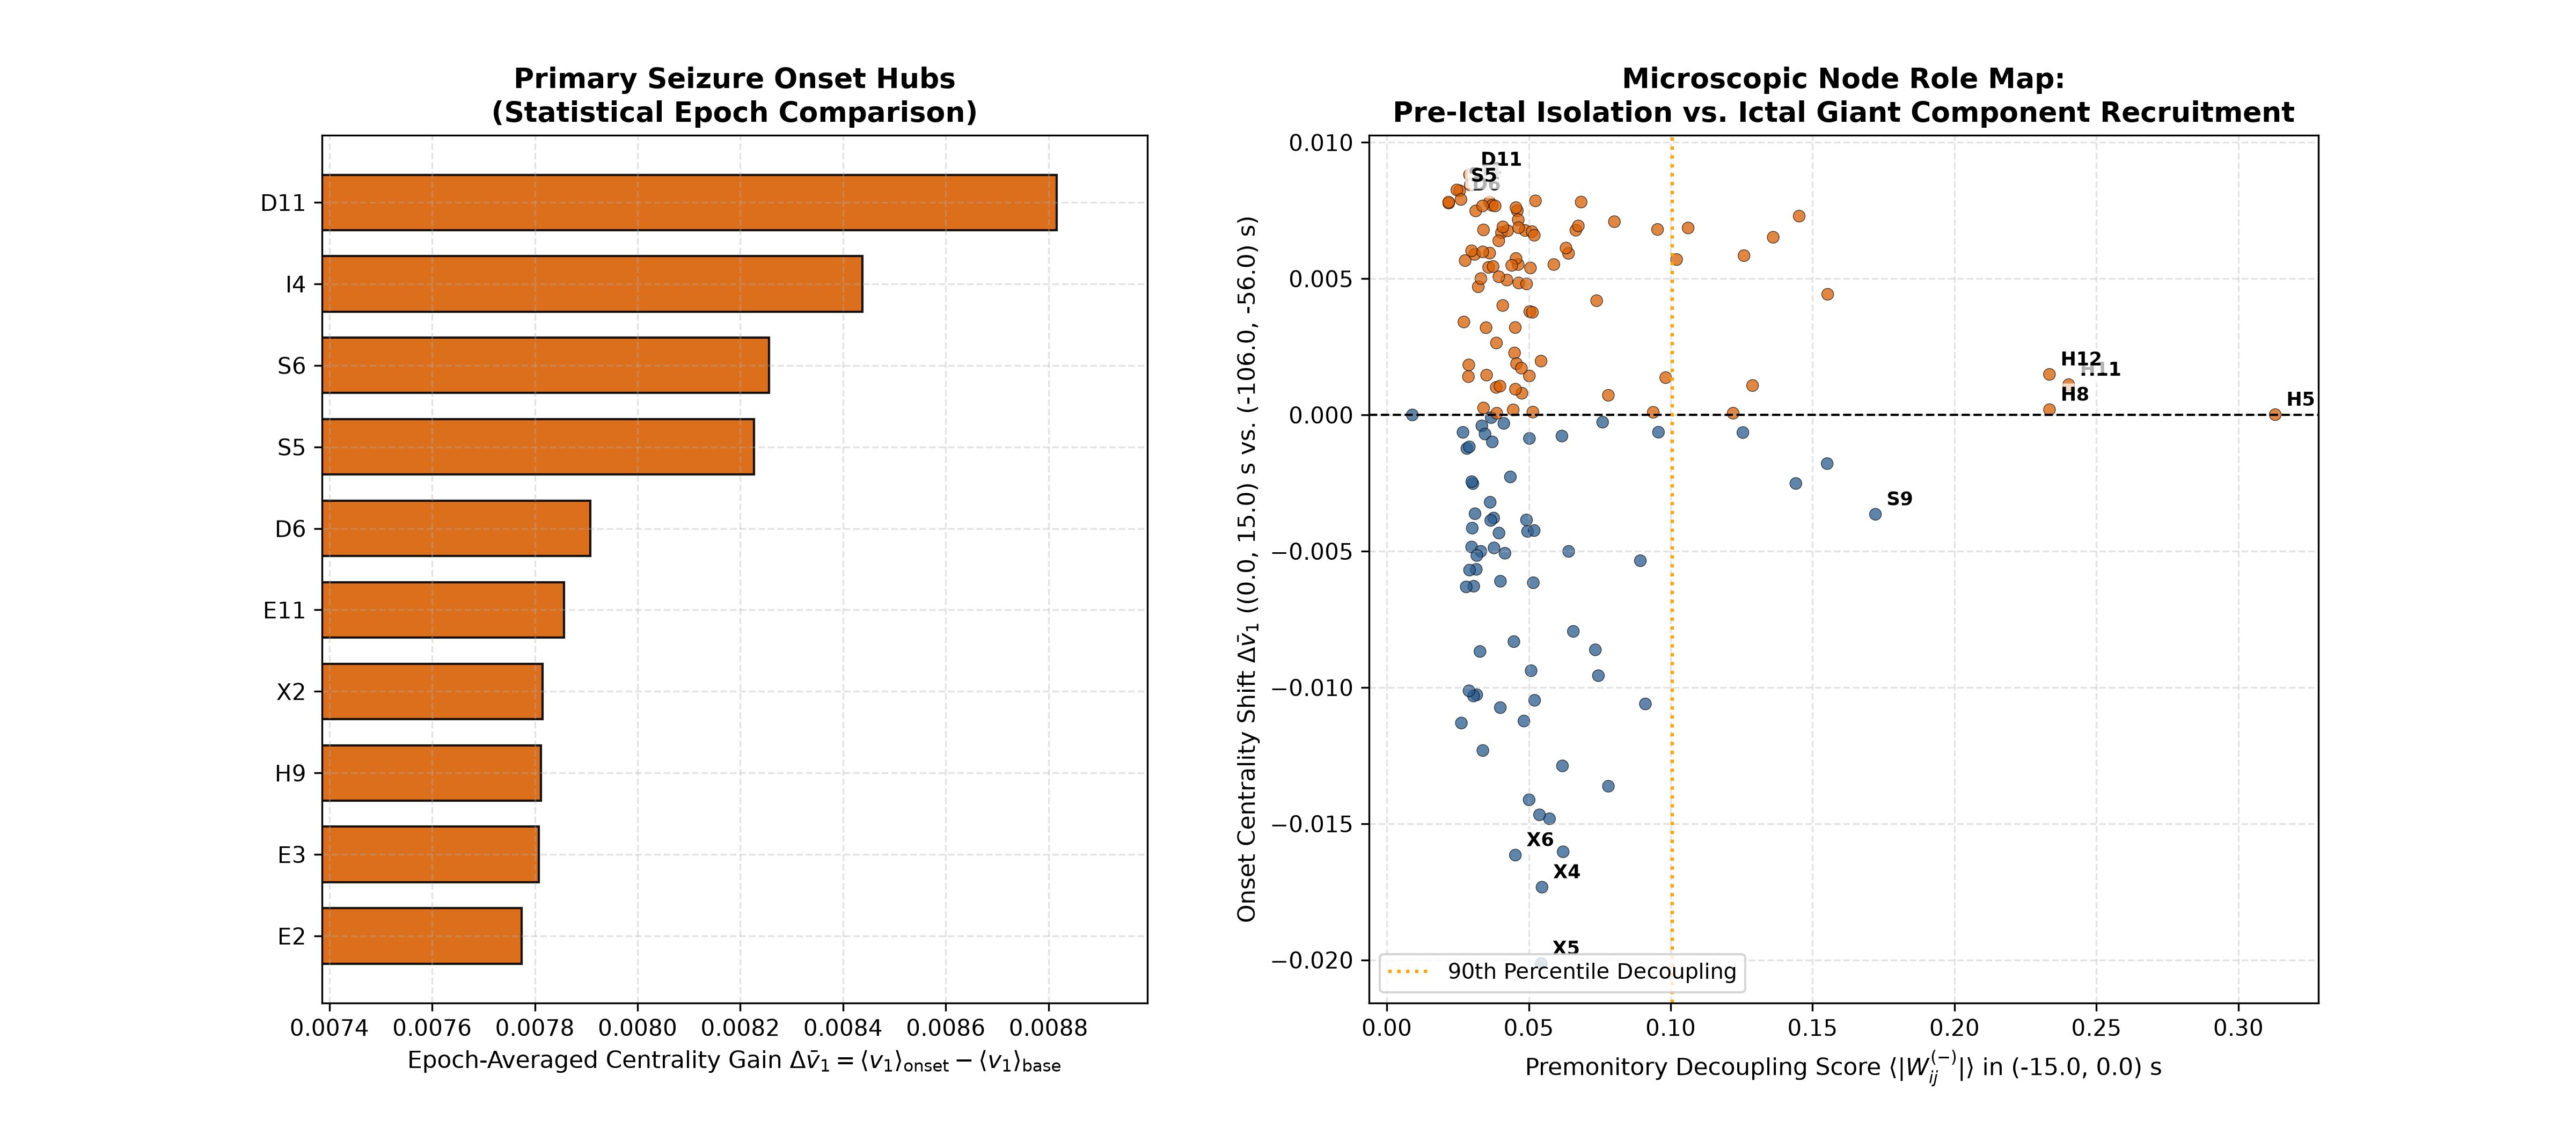
\includegraphics[width=0.9\textwidth]{img/DQ0040WG/micro_hub_recruitment_and_roles.png}
    \caption{Onset Hub Ranking and 2D Functional Role Map for recording \texttt{DQ0040WG}.}
    \label{fig:dq0040wg_micro_roles}
\end{figure}